\documentclass[11pt,a4paper]{article}
\usepackage[utf8]{inputenc}
\usepackage[T1]{fontenc}
\usepackage[polish]{babel}
\usepackage{amsmath,amssymb}
\usepackage{graphicx}
\usepackage{subcaption}
\usepackage{booktabs}
\usepackage{geometry}
\usepackage{hyperref}
\geometry{top=2.5cm,bottom=2.5cm,left=2.5cm,right=2.5cm}

% Ścieżka bazowa do wykresów (dostosuj do struktury katalogów swojego projektu)
\graphicspath{{plots/}}

\title{\textbf{Katalog Rysunków i Wzorców LaTeX dla Publikacji Local PCA}}
\author{Zespół Badawczy Atraktorów w QGP}
\date{25 września 2026}

\begin{document}
\maketitle

\tableofcontents
\newpage

\section{Wprowadzenie}
Wszystkie pliki PDF w niniejszym katalogu zostały wygenerowane \textbf{bez wewnętrznych tytułów}, co eliminuje redundancję wizualną i pozwala na pełną kontrolę nad opisem rysunku z poziomu środowiska \texttt{\textbackslash caption}. Ponadto dla siatek przestrzeni fazowych zastosowano schemat estymacji na gęstym zbiorze $N_{\text{calc}} = 10\,000$ punktów na plaster $\tau$ oraz prezentacji graficznej $N_{\text{plot}} = 5\,000$ punktów (zapobiegający zjawisku \emph{overplotting} w 2D i 3D oraz optymalizujący objętość plików wektorowych).

Poniżej przedstawiono gotowe do skopiowania bloki kodu dla wszystkich głównych kategorii rysunków.

\section{Kategoria I: Siatki ewolucji 2D i 3D}

\subsection{Model Conformal MIS (2D: $T, \mathcal{A}$)}

\begin{figure}[htbp]
    \centering
    % Wiersz 1: Dimensionless
    \begin{subfigure}[b]{0.48\textwidth}
        \centering
        \includegraphics[width=\linewidth]{best_practices_lpca/grid_mis_dimensionless_dims.pdf}
        \caption{Dimensionless (\emph{dims})}
        \label{fig:mis_dim_dims}
    \end{subfigure}
    \hfill
    \begin{subfigure}[b]{0.48\textwidth}
        \centering
        \includegraphics[width=\linewidth]{best_practices_lpca/grid_mis_dimensionless_pr.pdf}
        \caption{Dimensionless (\emph{pr})}
        \label{fig:mis_dim_pr}
    \end{subfigure}

    \vspace{0.8em}

    % Wiersz 2: Max
    \begin{subfigure}[b]{0.48\textwidth}
        \centering
        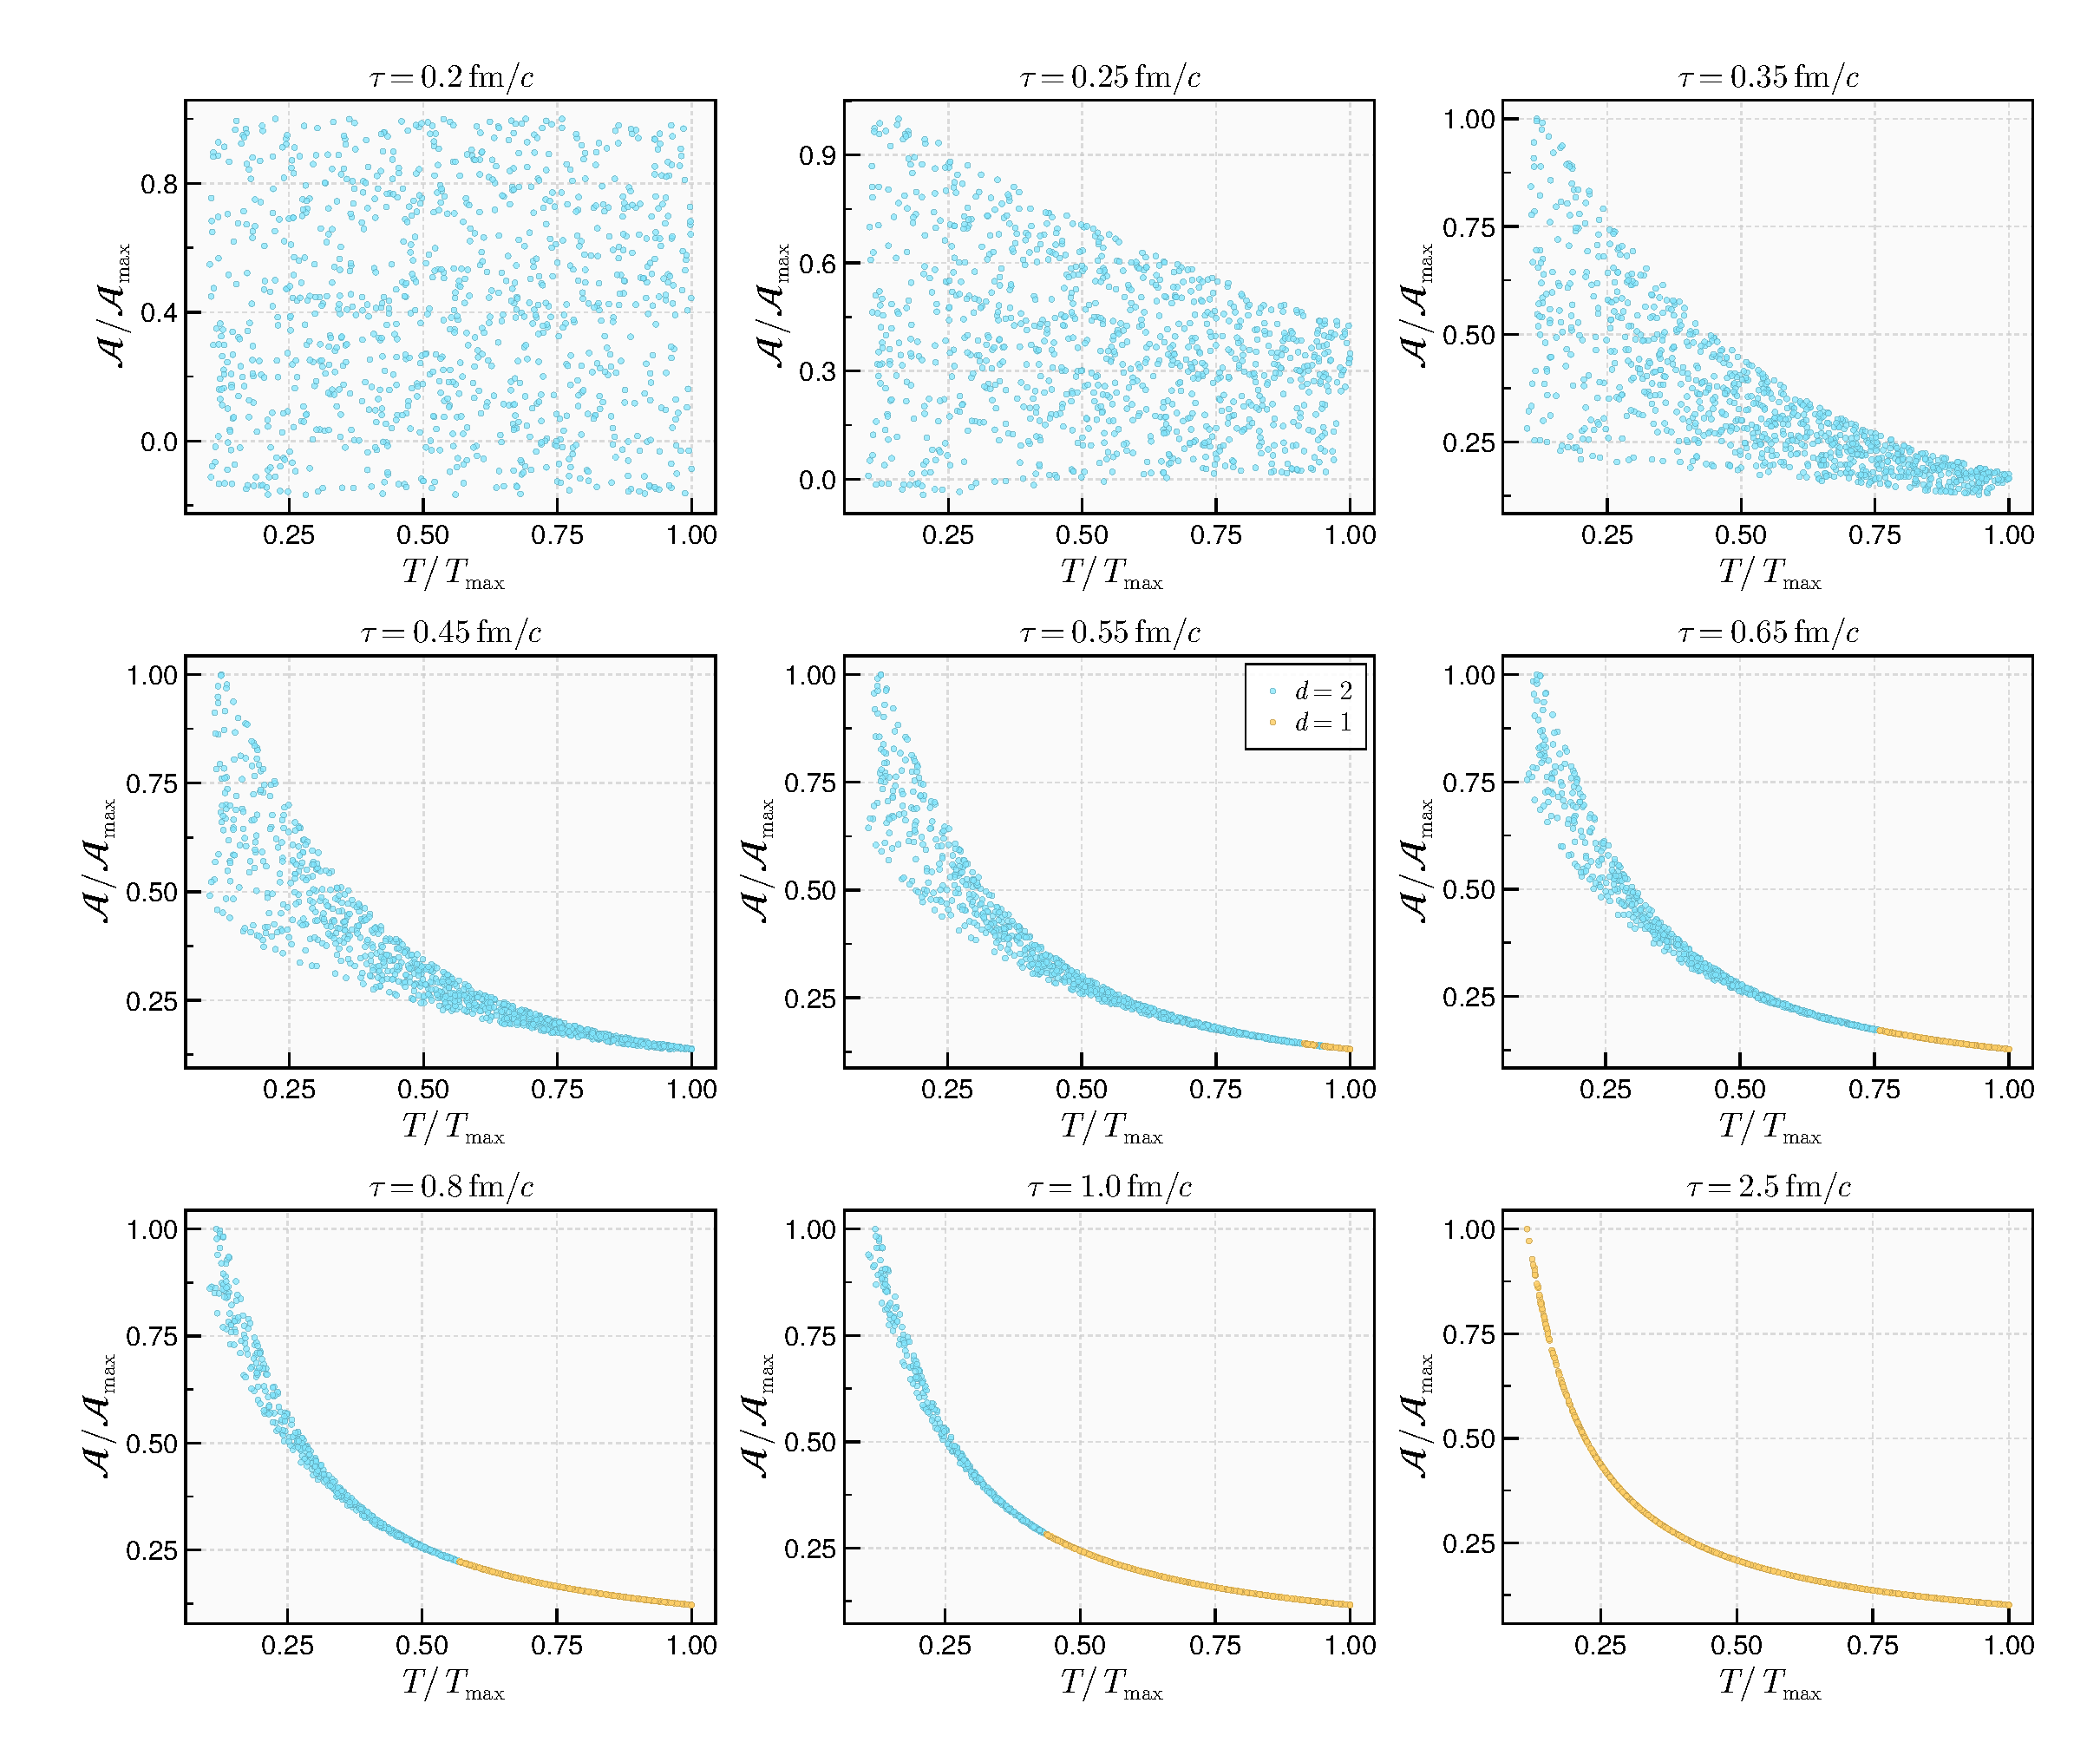
\includegraphics[width=\linewidth]{best_practices_lpca/grid_mis_max_dims.pdf}
        \caption{Abs-Max (\emph{dims})}
        \label{fig:mis_max_dims}
    \end{subfigure}
    \hfill
    \begin{subfigure}[b]{0.48\textwidth}
        \centering
        \includegraphics[width=\linewidth]{best_practices_lpca/grid_mis_max_pr.pdf}
        \caption{Abs-Max (\emph{pr})}
        \label{fig:mis_max_pr}
    \end{subfigure}

    \caption{Ewolucja przestrzeni fazowej w modelu Conformal MIS (cz.~1): lewa kolumna przedstawia dyskretny wymiar lokalny \emph{dims} ($\text{tol}=0.01$), prawa wskaźnik ciągły Participation Ratio \emph{pr}. Pierwszy panel odpowiada stanowi początkowemu $\tau_0 = 0.20\,\mathrm{fm}/c$.}
    \label{fig:mis_phase_space_part1}
\end{figure}

\begin{figure}[htbp]\ContinuedFloat
    \centering
    % Wiersz 3: Min-Max
    \begin{subfigure}[b]{0.48\textwidth}
        \centering
        \includegraphics[width=\linewidth]{best_practices_lpca/grid_mis_minmax_dims.pdf}
        \caption{Min-Max (\emph{dims})}
        \label{fig:mis_minmax_dims}
    \end{subfigure}
    \hfill
    \begin{subfigure}[b]{0.48\textwidth}
        \centering
        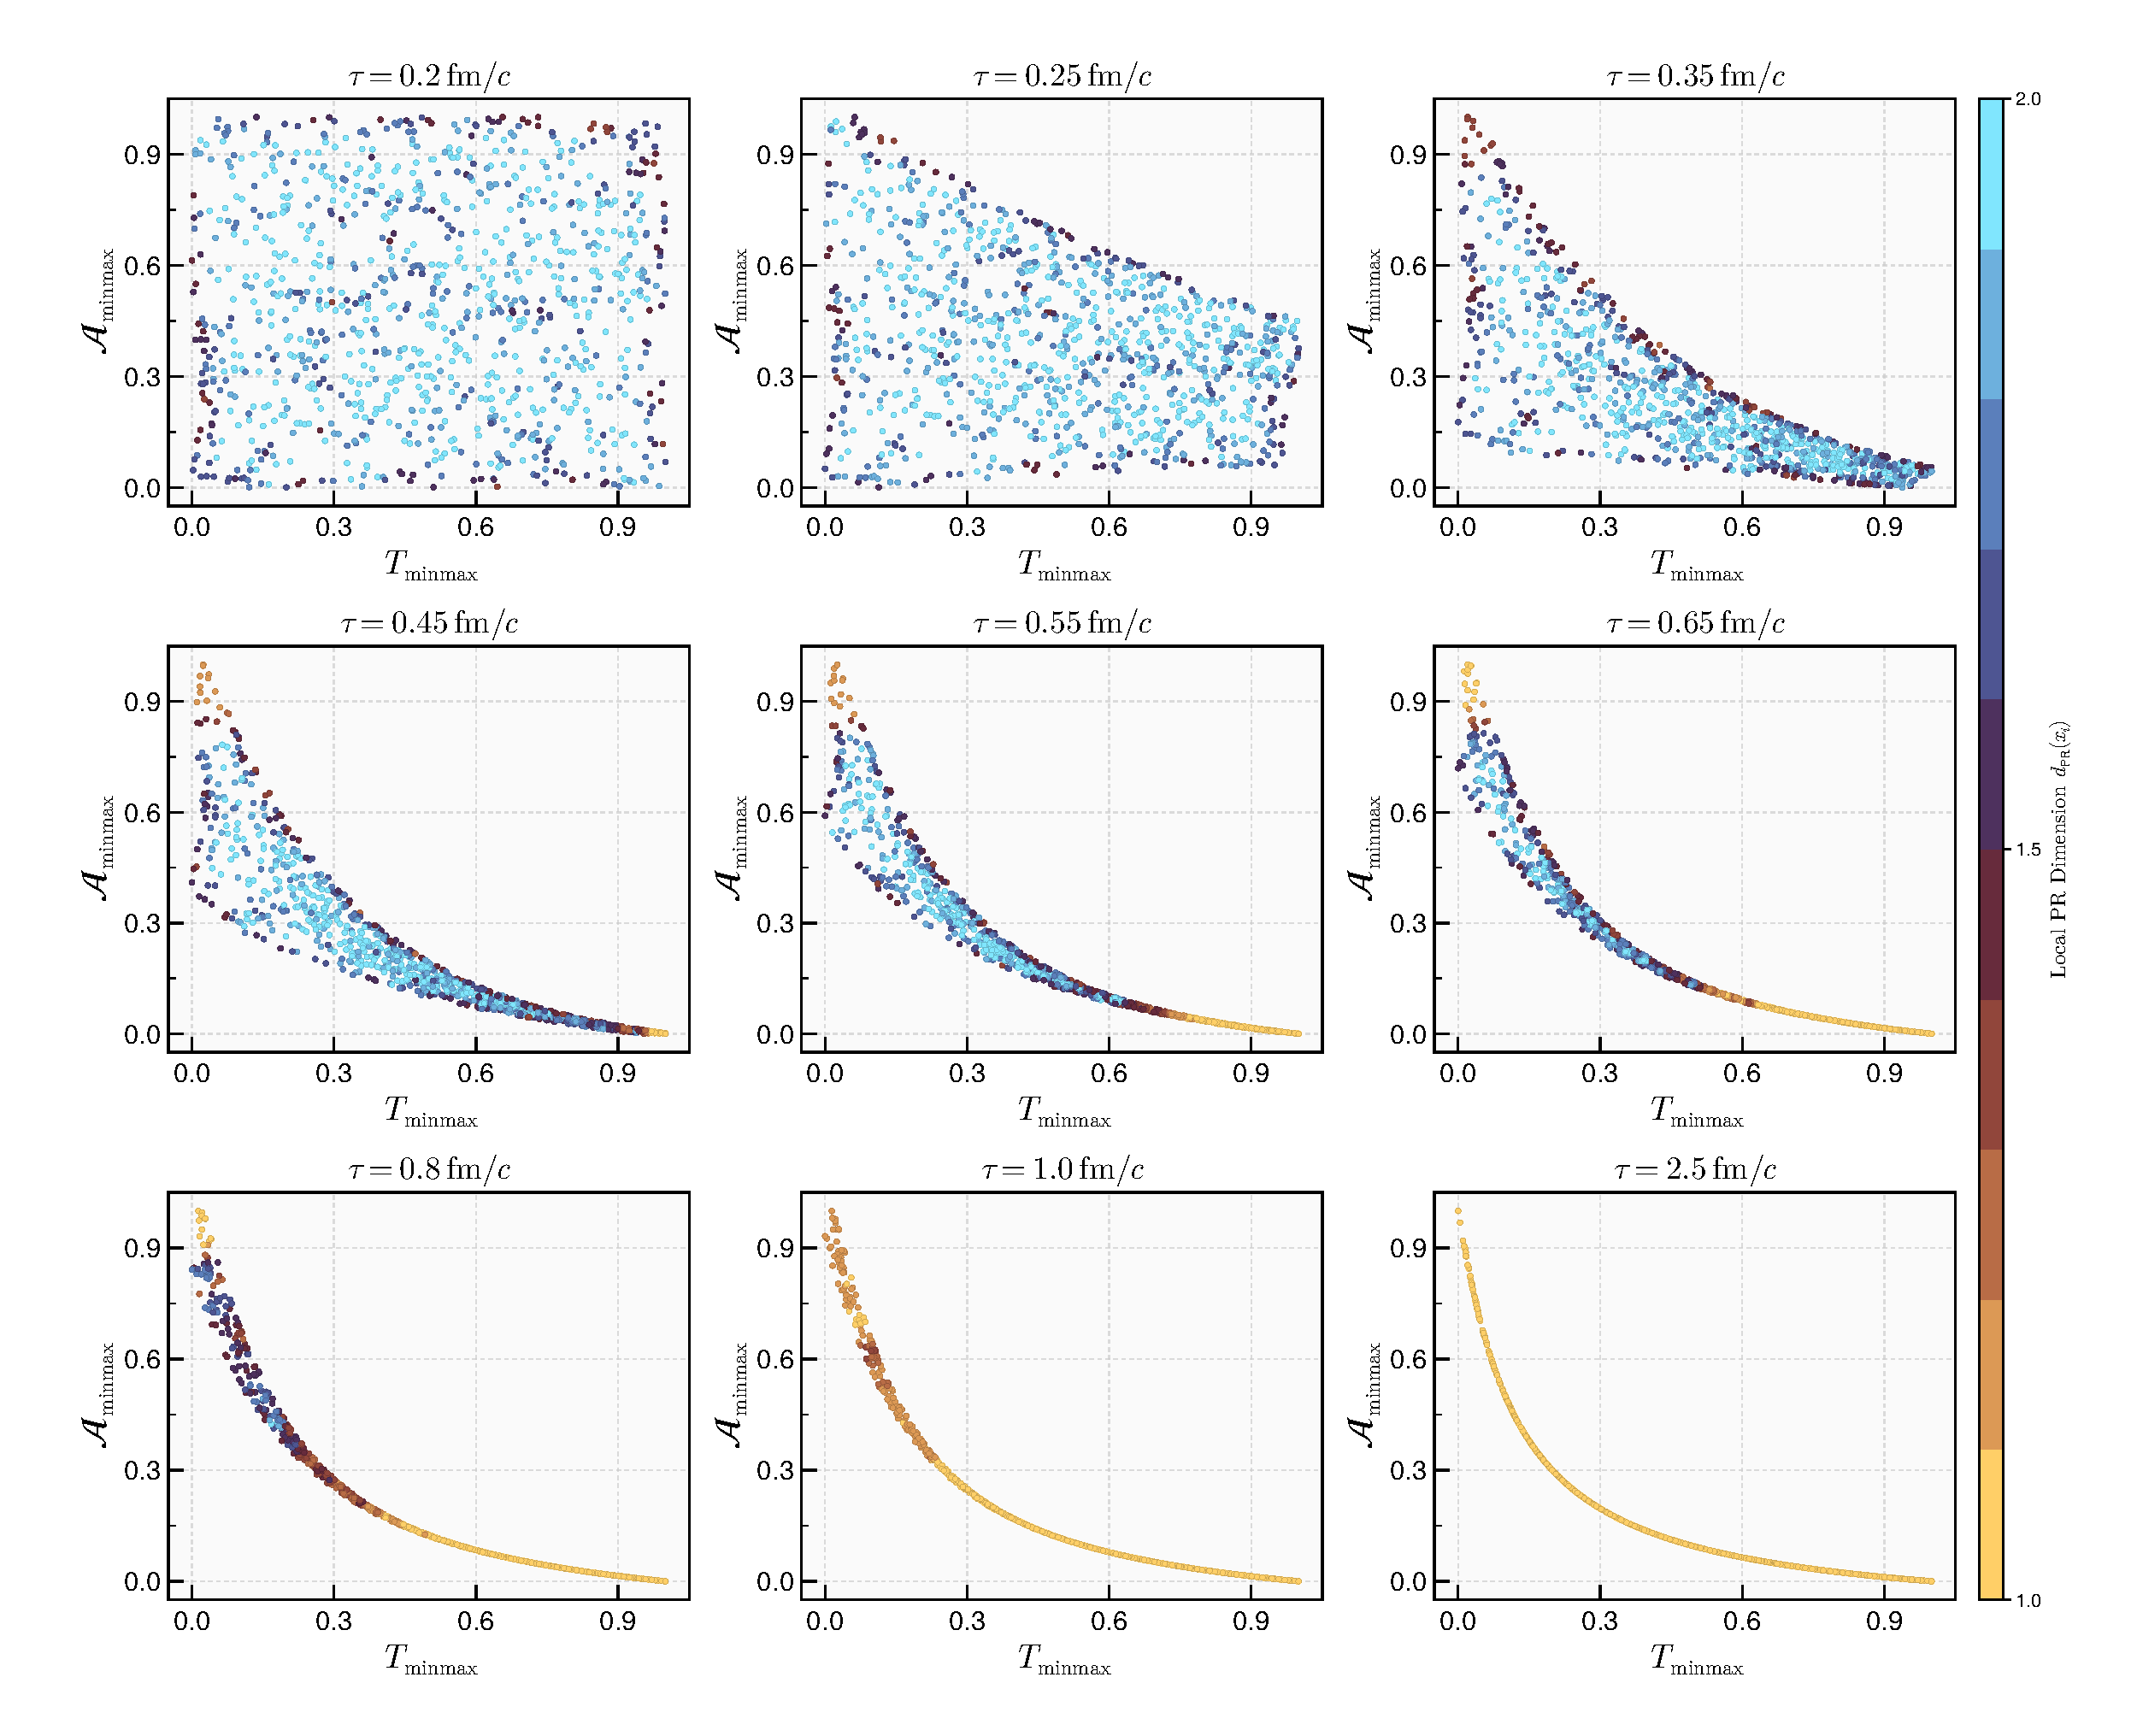
\includegraphics[width=\linewidth]{best_practices_lpca/grid_mis_minmax_pr.pdf}
        \caption{Min-Max (\emph{pr})}
        \label{fig:mis_minmax_pr}
    \end{subfigure}

    \vspace{0.8em}

    % Wiersz 4: Z-Score
    \begin{subfigure}[b]{0.48\textwidth}
        \centering
        \includegraphics[width=\linewidth]{best_practices_lpca/grid_mis_zscore_dims.pdf}
        \caption{Z-Score (\emph{dims})}
        \label{fig:mis_zscore_dims}
    \end{subfigure}
    \hfill
    \begin{subfigure}[b]{0.48\textwidth}
        \centering
        \includegraphics[width=\linewidth]{best_practices_lpca/grid_mis_zscore_pr.pdf}
        \caption{Z-Score (\emph{pr})}
        \label{fig:mis_zscore_pr}
    \end{subfigure}

    \caption{Ewolucja przestrzeni fazowej w modelu Conformal MIS (cz.~2, dokończenie): warianty Min-Max oraz Z-Score.}
    \label{fig:mis_phase_space_part2}
\end{figure}

\clearpage
\subsection{Model HJSW (3D: $T, \mathcal{A}, \mathcal{B}$)}

\begin{figure}[htbp]
    \centering
    \begin{subfigure}[b]{0.48\textwidth}
        \centering
        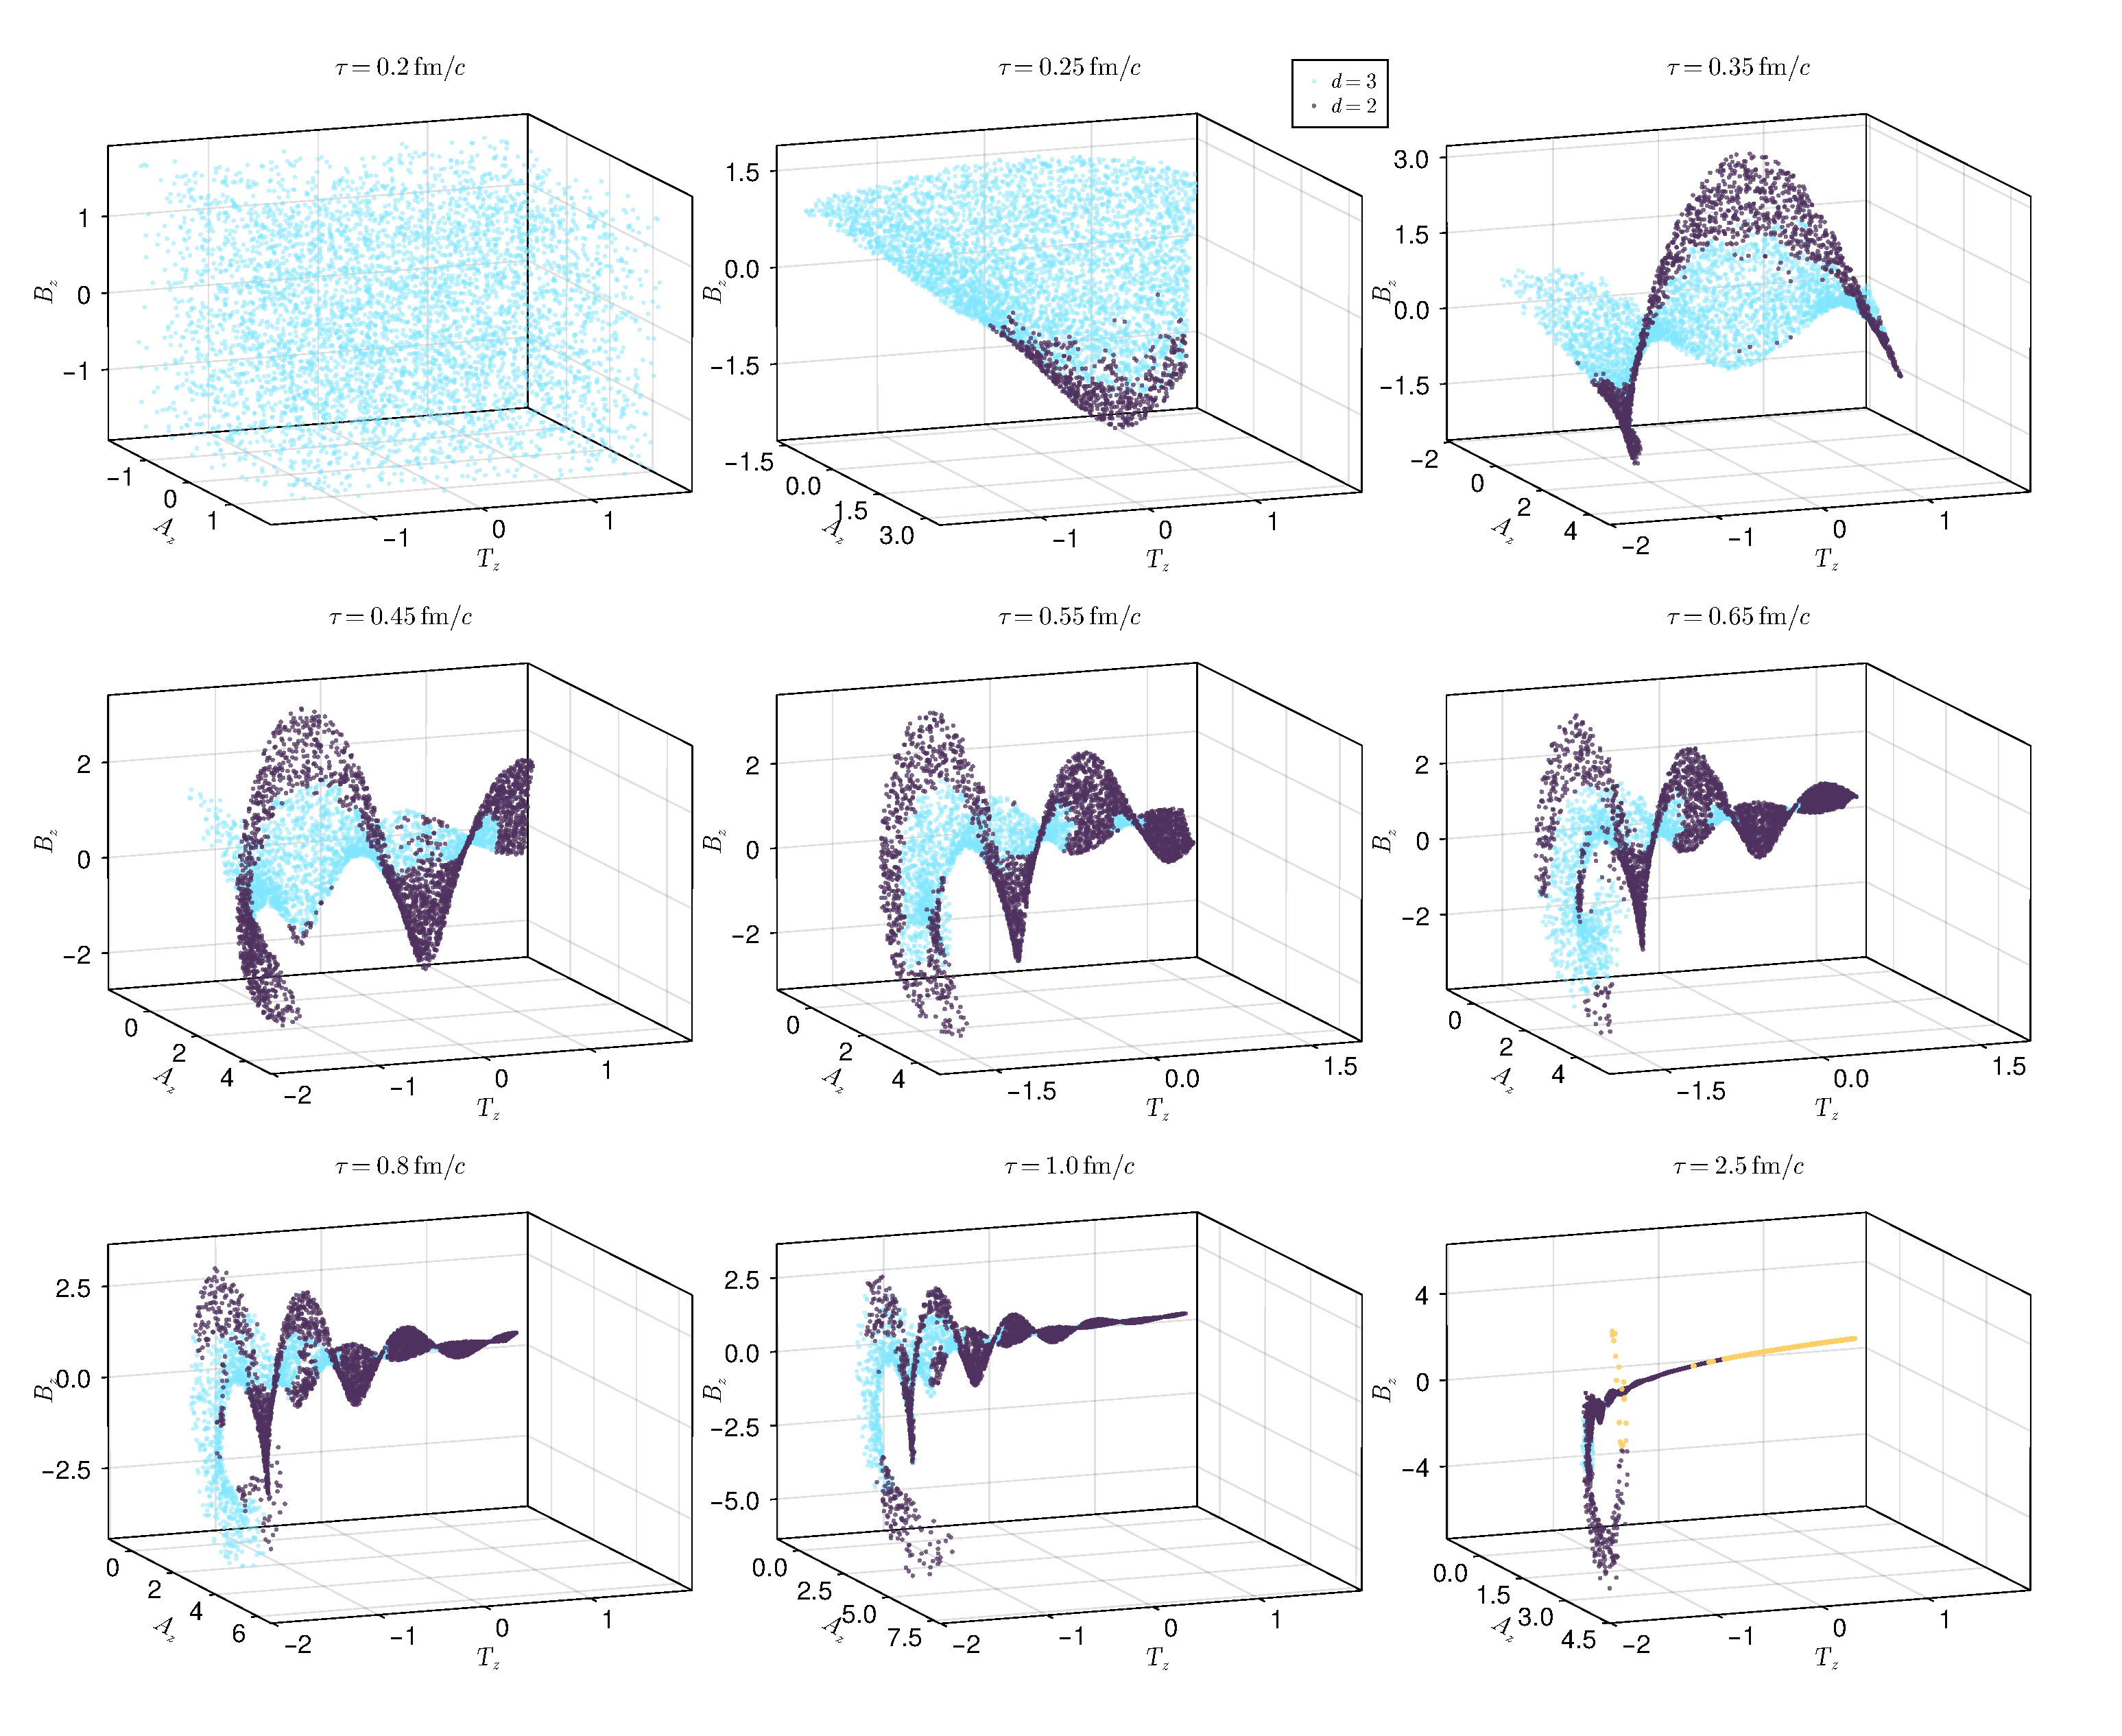
\includegraphics[width=\linewidth]{best_practices_lpca/grid_hjsw_zscore_dims.pdf}
        \caption{HJSW Z-Score (\emph{dims})}
        \label{fig:hjsw_zscore_dims}
    \end{subfigure}
    \hfill
    \begin{subfigure}[b]{0.48\textwidth}
        \centering
        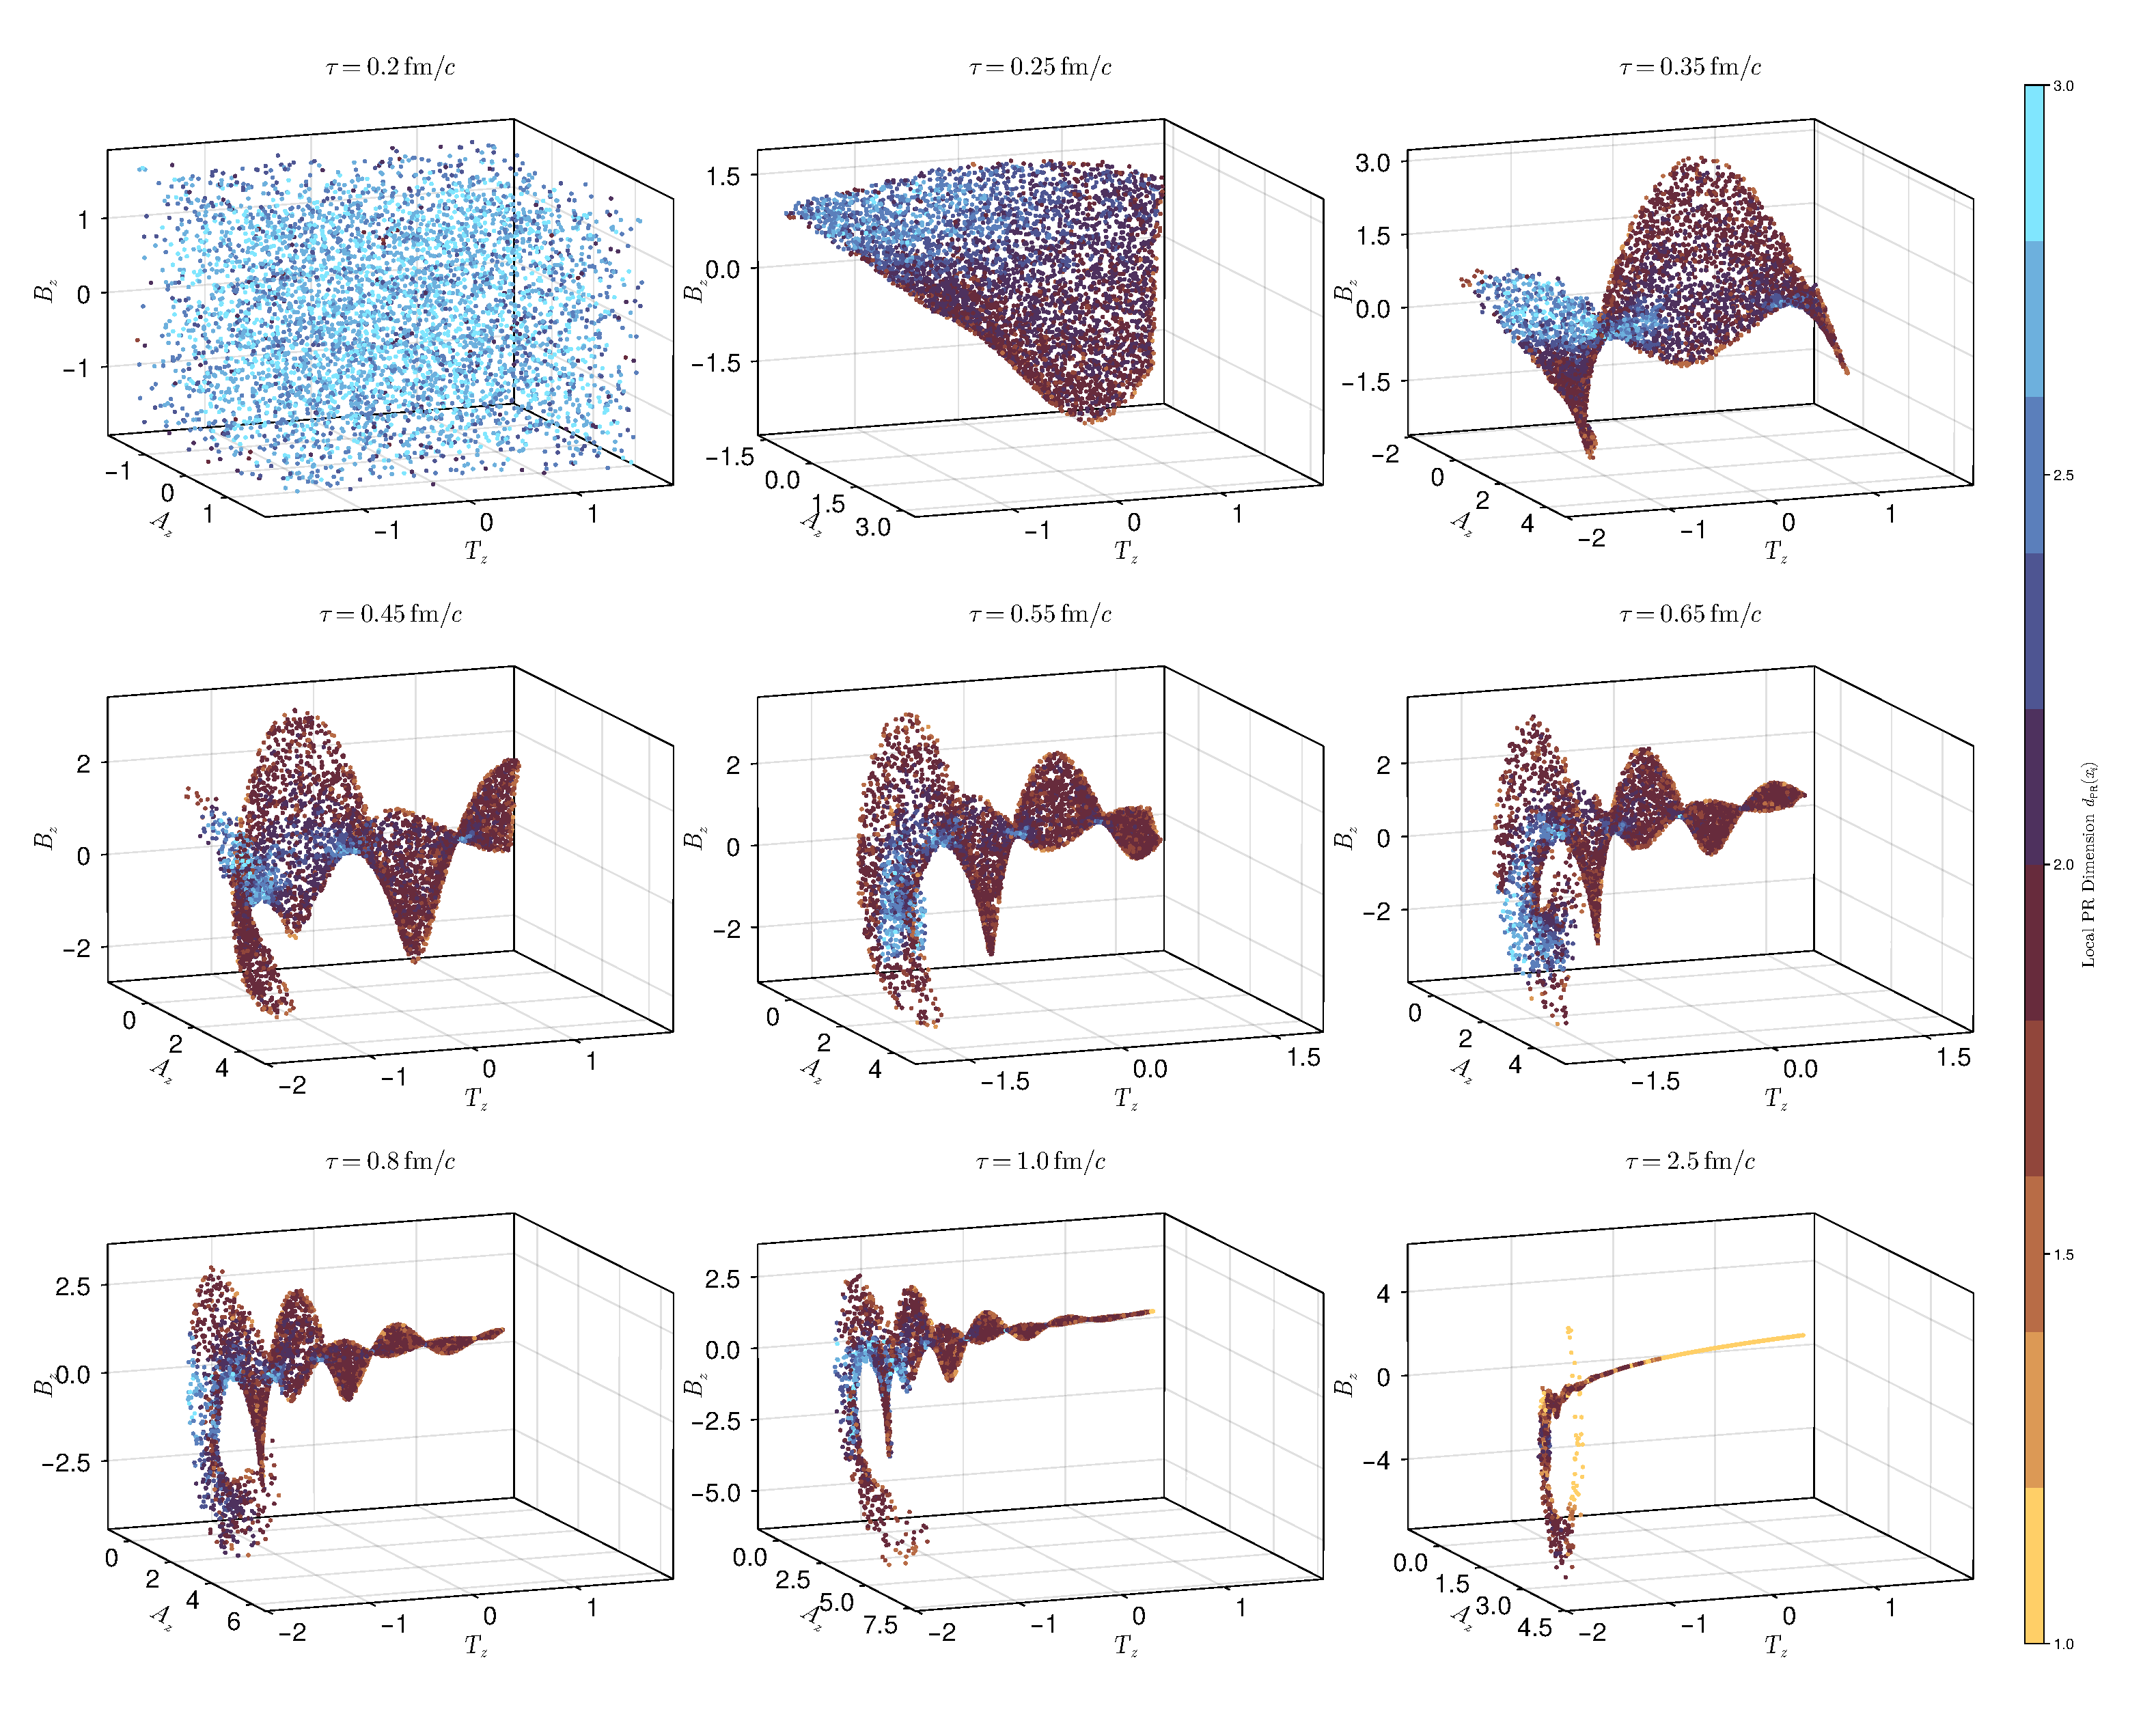
\includegraphics[width=\linewidth]{best_practices_lpca/grid_hjsw_zscore_pr.pdf}
        \caption{HJSW Z-Score (\emph{pr})}
        \label{fig:hjsw_zscore_pr}
    \end{subfigure}

    \caption{Hierarchiczny kolaps wymiarowości $3 \to 2 \to 1$ w modelu HJSW w standaryzacji Z-Score. W chwili $\tau_0 = 0.20\,\mathrm{fm}/c$ układ wypełnia pełną przestrzeń 3D. W $\tau = 0.25\,\mathrm{fm}/c$ szybki mod niehydrodynamiczny ulega kompresji 58-krotnej, wprowadzając układ w 2-wymiarową rozmaitość pośrednią ($d \approx 2.0$), która następnie wolno kolapsuje hydrodynamicznie ku 1D atraktorowi.}
    \label{fig:hjsw_phase_space_zscore}
\end{figure}

\clearpage
\section{Kategoria II: Ewolucja wymiaru w czasie $d(\tau)$ dla $K \in [3, 50]$}

\subsection{Wariant z czystymi liniami (Lines Only -- bez pasm błędu)}

\begin{figure}[htbp]
    \centering
    \begin{subfigure}[b]{0.48\textwidth}
        \centering
        \includegraphics[width=\linewidth]{d_vs_tau_k_dependency/d_vs_tau_mis_multi_k_lines_dims.pdf}
        \caption{MIS: \emph{dims} ($K \in [3, 50]$)}
        \label{fig:d_tau_mis_lines_dims}
    \end{subfigure}
    \hfill
    \begin{subfigure}[b]{0.48\textwidth}
        \centering
        \includegraphics[width=\linewidth]{d_vs_tau_k_dependency/d_vs_tau_mis_multi_k_lines_pr.pdf}
        \caption{MIS: \emph{pr} ($K \in [3, 50]$)}
        \label{fig:d_tau_mis_lines_pr}
    \end{subfigure}

    \vspace{0.8em}

    \begin{subfigure}[b]{0.48\textwidth}
        \centering
        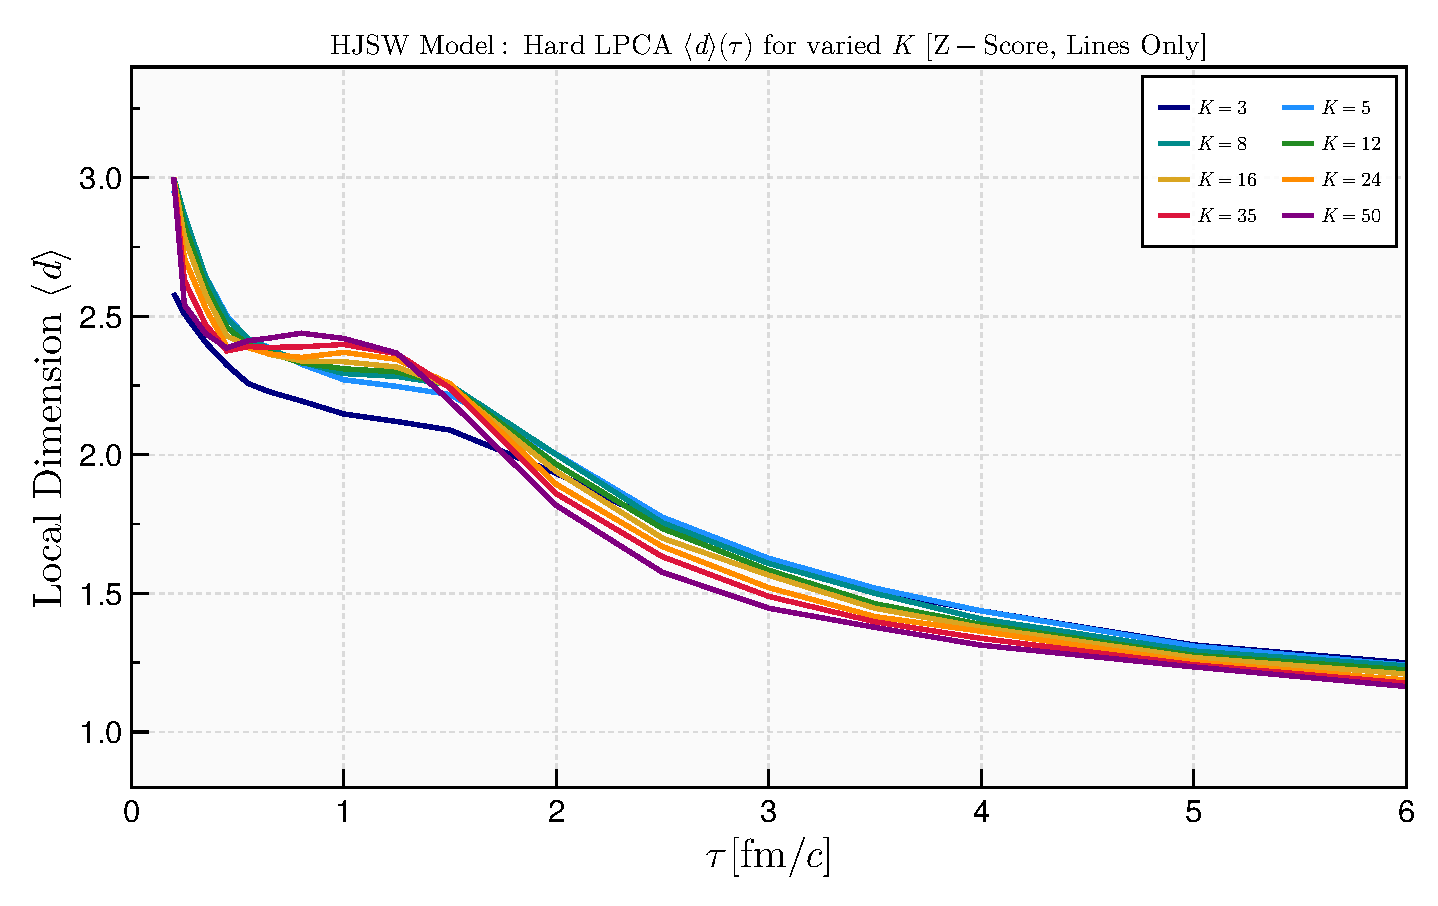
\includegraphics[width=\linewidth]{d_vs_tau_k_dependency/d_vs_tau_hjsw_multi_k_lines_dims.pdf}
        \caption{HJSW: \emph{dims} ($K \in [3, 50]$)}
        \label{fig:d_tau_hjsw_lines_dims}
    \end{subfigure}
    \hfill
    \begin{subfigure}[b]{0.48\textwidth}
        \centering
        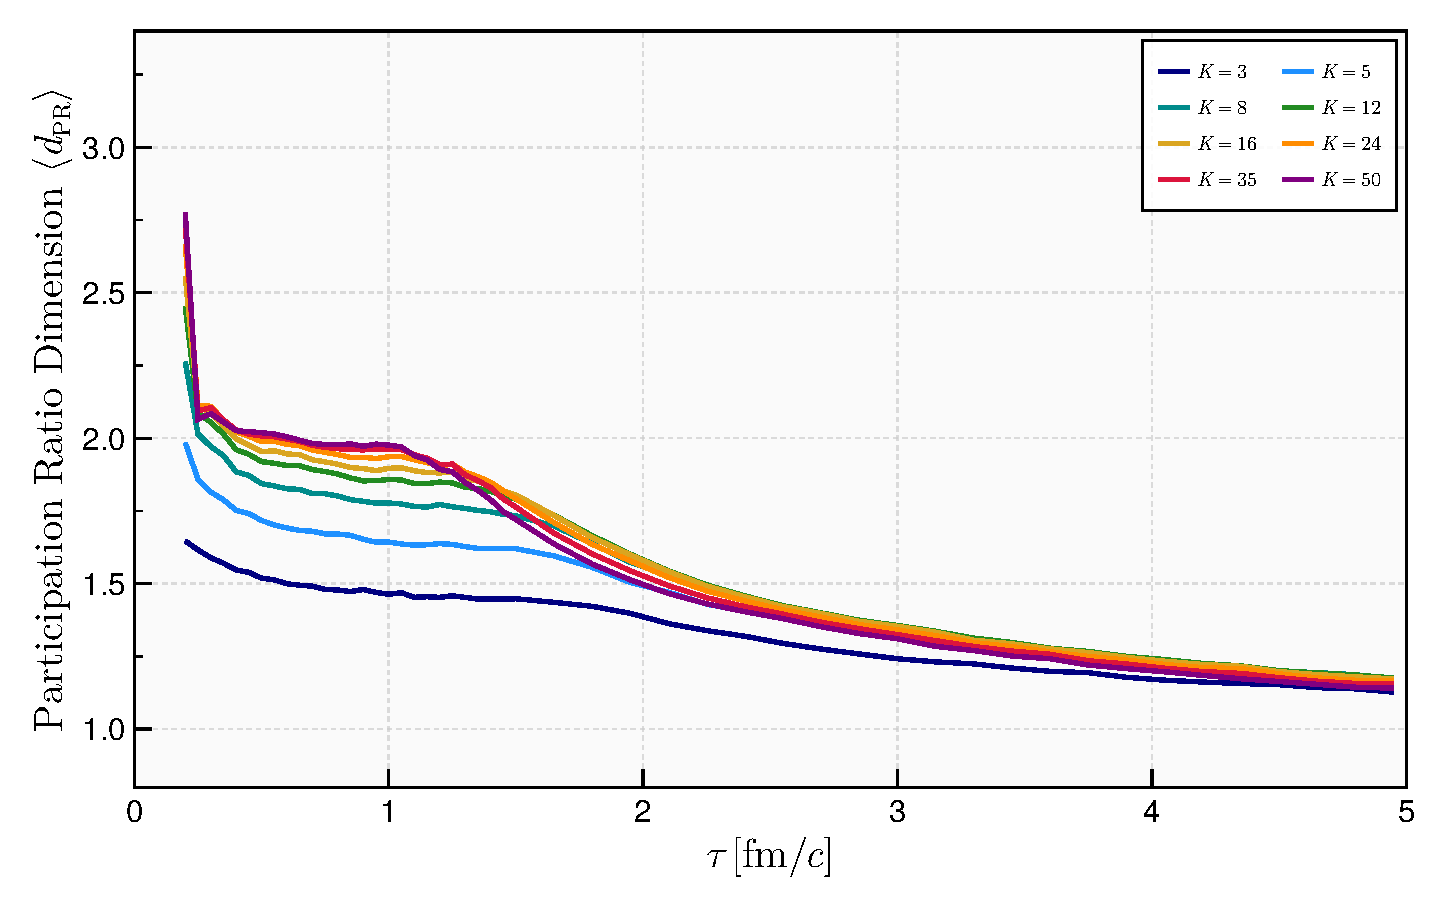
\includegraphics[width=\linewidth]{d_vs_tau_k_dependency/d_vs_tau_hjsw_multi_k_lines_pr.pdf}
        \caption{HJSW: \emph{pr} ($K \in [3, 50]$)}
        \label{fig:d_tau_hjsw_lines_pr}
    \end{subfigure}

    \caption{Trajektorie ewolucji wymiaru $d(\tau)$ dla wybranych wartości $K \in \{3, 5, 8, 12, 16, 24, 35, 50\}$ (standaryzacja Z-Score). Wariant \emph{Lines Only} bez pasm błędu ukazuje, że dla dowolnego $K \ge 12$ krzywe leżą niemal dokładnie na sobie, co dowodzi niezmienniczości wyznaczanego wymiaru względem skali $k$-NN.}
    \label{fig:d_vs_tau_multi_k_lines}
\end{figure}

\subsection{Wariant uśredniony po $K \in [3, 50]$ z pasmem niepewności $\pm 1\sigma_K$}

\begin{figure}[htbp]
    \centering
    \begin{subfigure}[b]{0.48\textwidth}
        \centering
        \includegraphics[width=\linewidth]{d_vs_tau_k_dependency/d_vs_tau_mis_k_averaged_dims.pdf}
        \caption{MIS: Średnia $\langle d \rangle_K$ (\emph{dims})}
        \label{fig:d_tau_mis_avg_dims}
    \end{subfigure}
    \hfill
    \begin{subfigure}[b]{0.48\textwidth}
        \centering
        \includegraphics[width=\linewidth]{d_vs_tau_k_dependency/d_vs_tau_mis_k_averaged_pr.pdf}
        \caption{MIS: Średnia $\langle d_{\mathrm{PR}} \rangle_K$ (\emph{pr})}
        \label{fig:d_tau_mis_avg_pr}
    \end{subfigure}

    \vspace{0.8em}

    \begin{subfigure}[b]{0.48\textwidth}
        \centering
        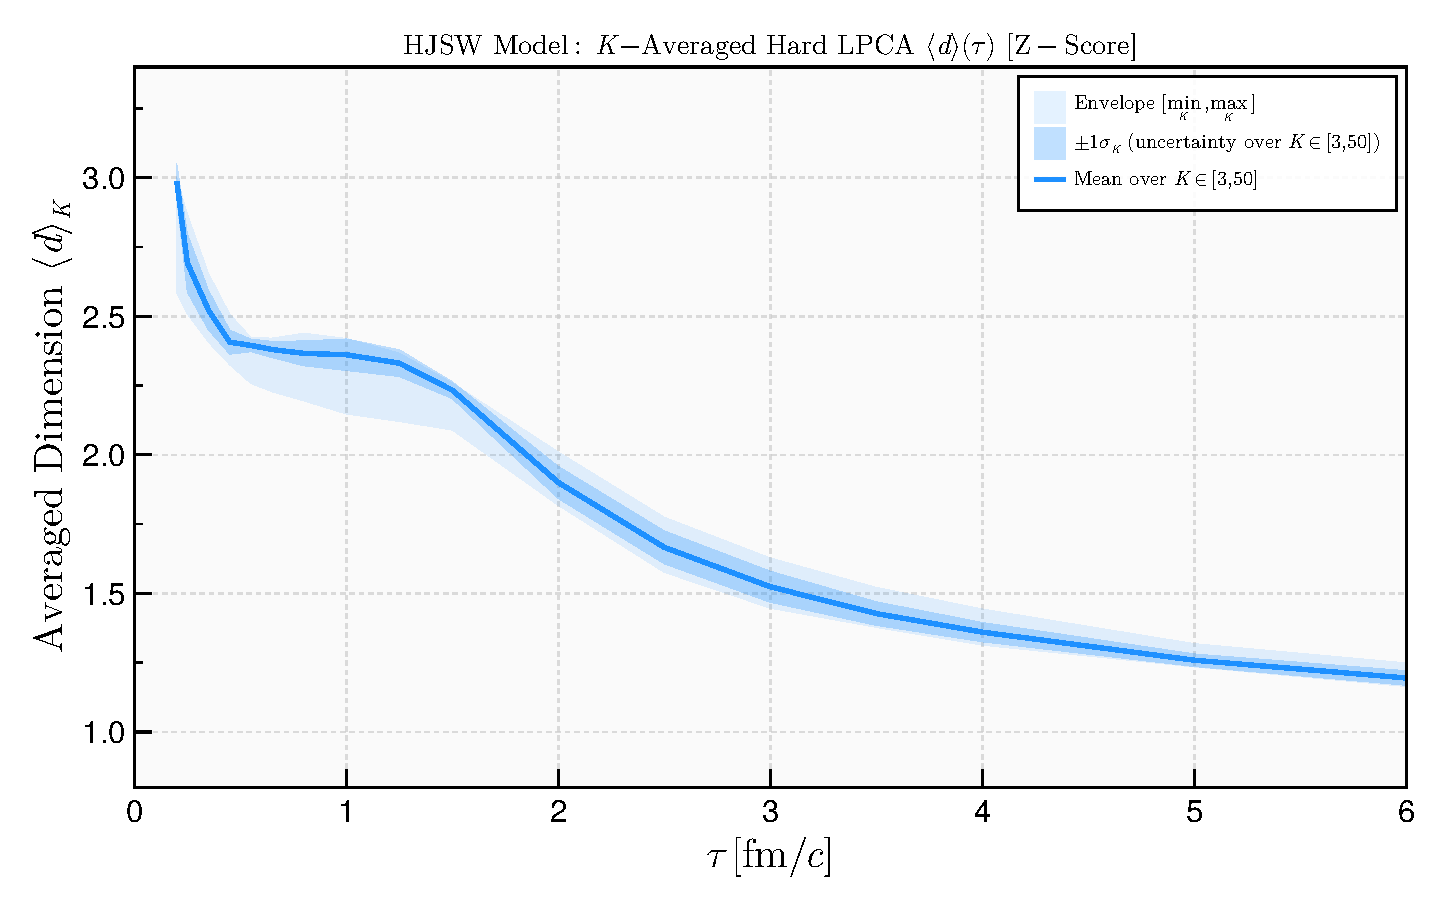
\includegraphics[width=\linewidth]{d_vs_tau_k_dependency/d_vs_tau_hjsw_k_averaged_dims.pdf}
        \caption{HJSW: Średnia $\langle d \rangle_K$ (\emph{dims})}
        \label{fig:d_tau_hjsw_avg_dims}
    \end{subfigure}
    \hfill
    \begin{subfigure}[b]{0.48\textwidth}
        \centering
        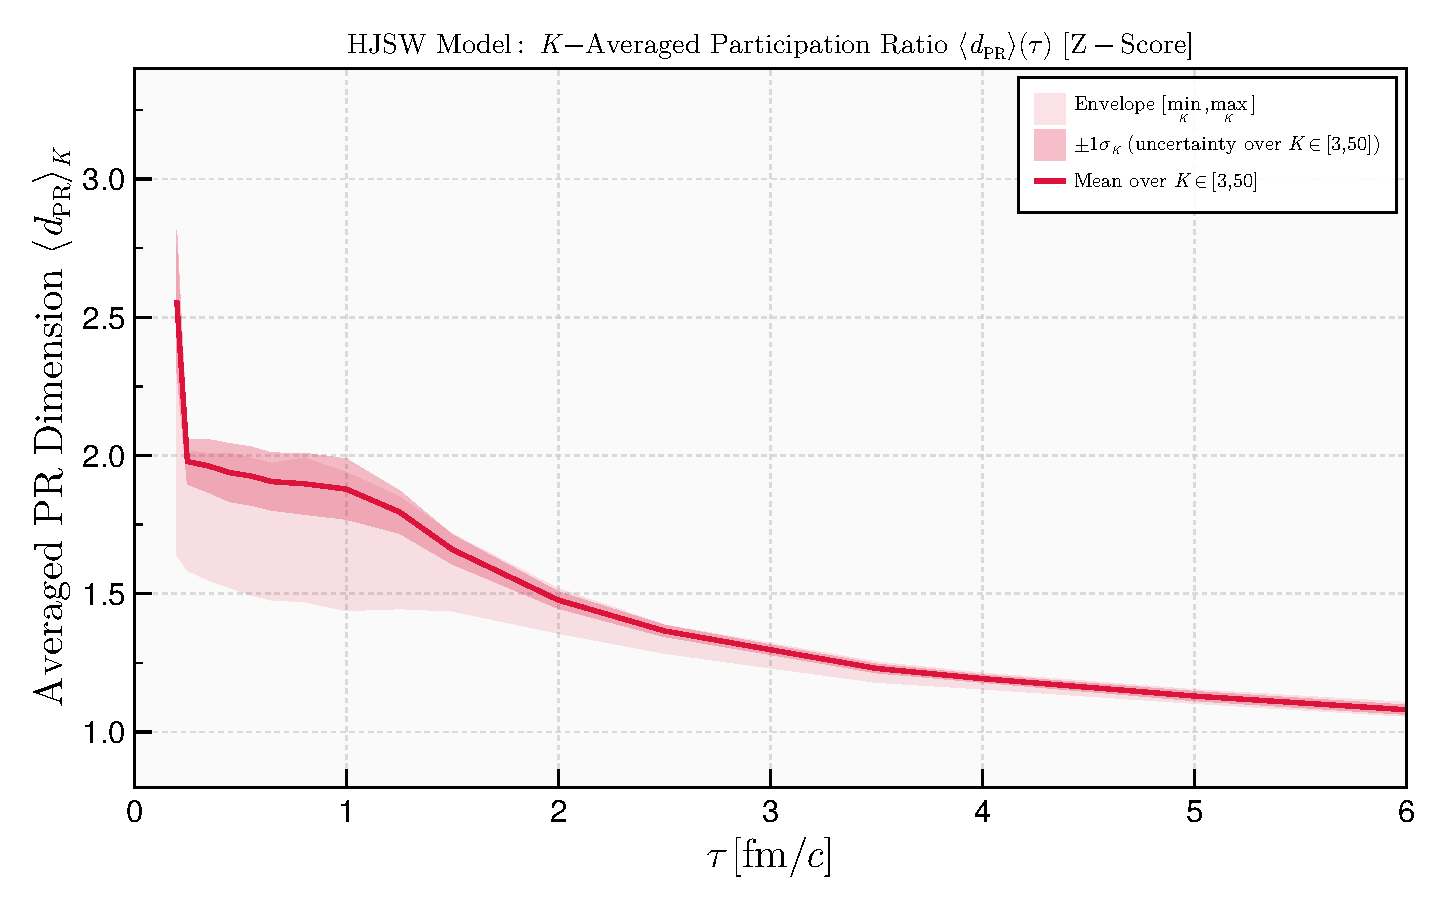
\includegraphics[width=\linewidth]{d_vs_tau_k_dependency/d_vs_tau_hjsw_k_averaged_pr.pdf}
        \caption{HJSW: Średnia $\langle d_{\mathrm{PR}} \rangle_K$ (\emph{pr})}
        \label{fig:d_tau_hjsw_avg_pr}
    \end{subfigure}

    \caption{Trajektoria ewolucji wymiaru uśredniona po pełnym zakresie $K \in [3, 50]$. Ciemniejsze pasmo reprezentuje niepewność arbitralnego doboru sąsiadów $\pm 1\sigma_K$, a jaśniejsze obwiednię $[\min_K, \max_K]$. Wąskość pasma potwierdza minimalny wpływ wyboru parametru $K$ na ostateczne wnioski fizyczne.}
    \label{fig:d_vs_tau_k_averaged}
\end{figure}

\subsection{Porównanie metod standaryzacji danych dla ewolucji $\langle d \rangle_K(\tau)$}

\begin{figure}[htbp]
    \centering
    \begin{subfigure}[b]{0.32\textwidth}
        \centering
        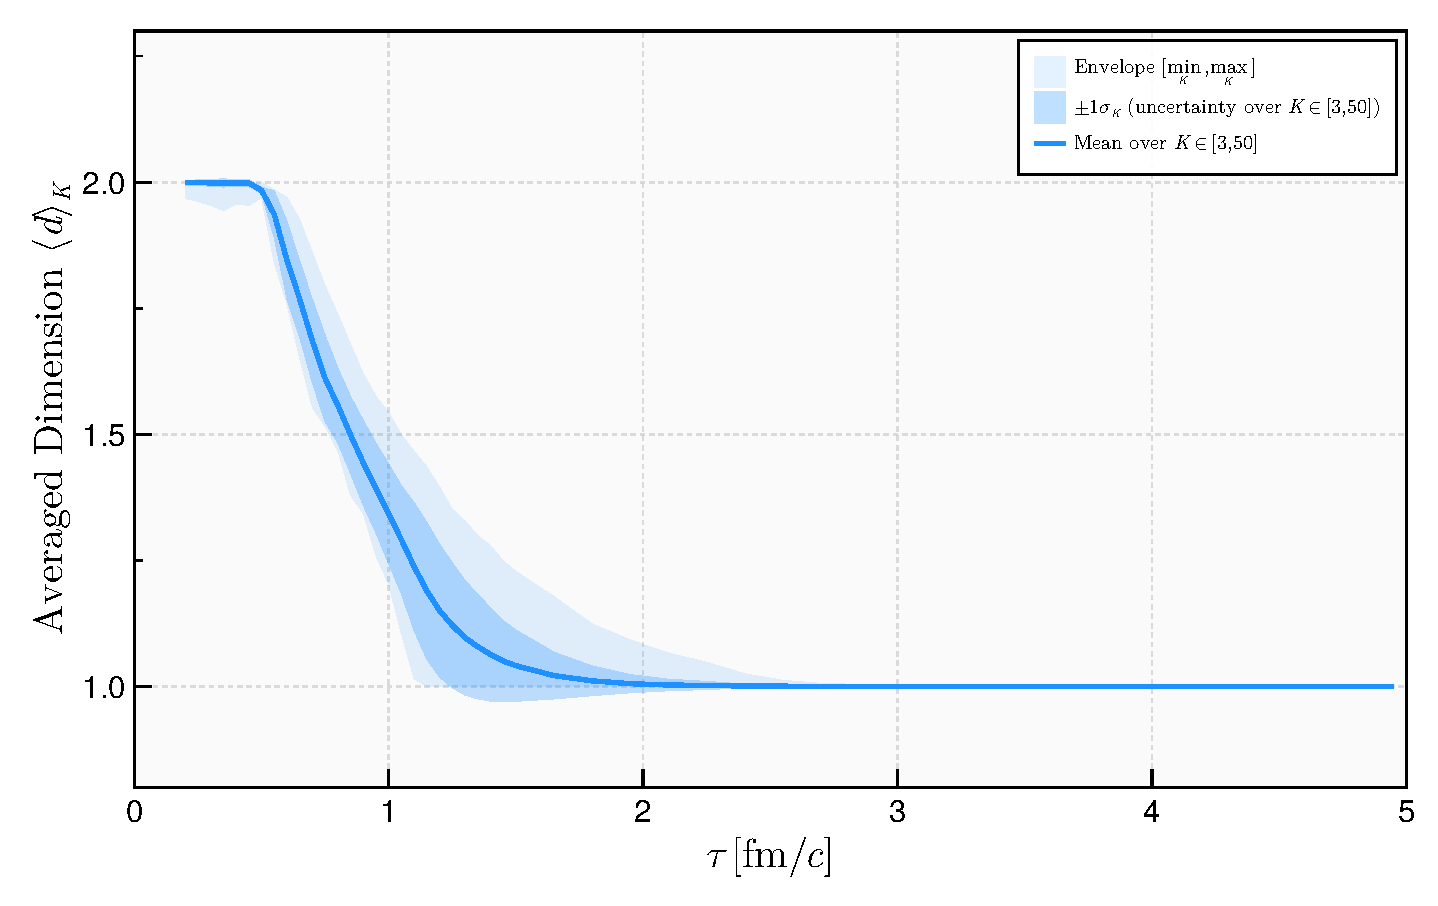
\includegraphics[width=\linewidth]{d_vs_tau_k_dependency/d_vs_tau_mis_zscore_k_averaged_dims.pdf}
        \caption{MIS: Z-Score}
    \end{subfigure}
    \hfill
    \begin{subfigure}[b]{0.32\textwidth}
        \centering
        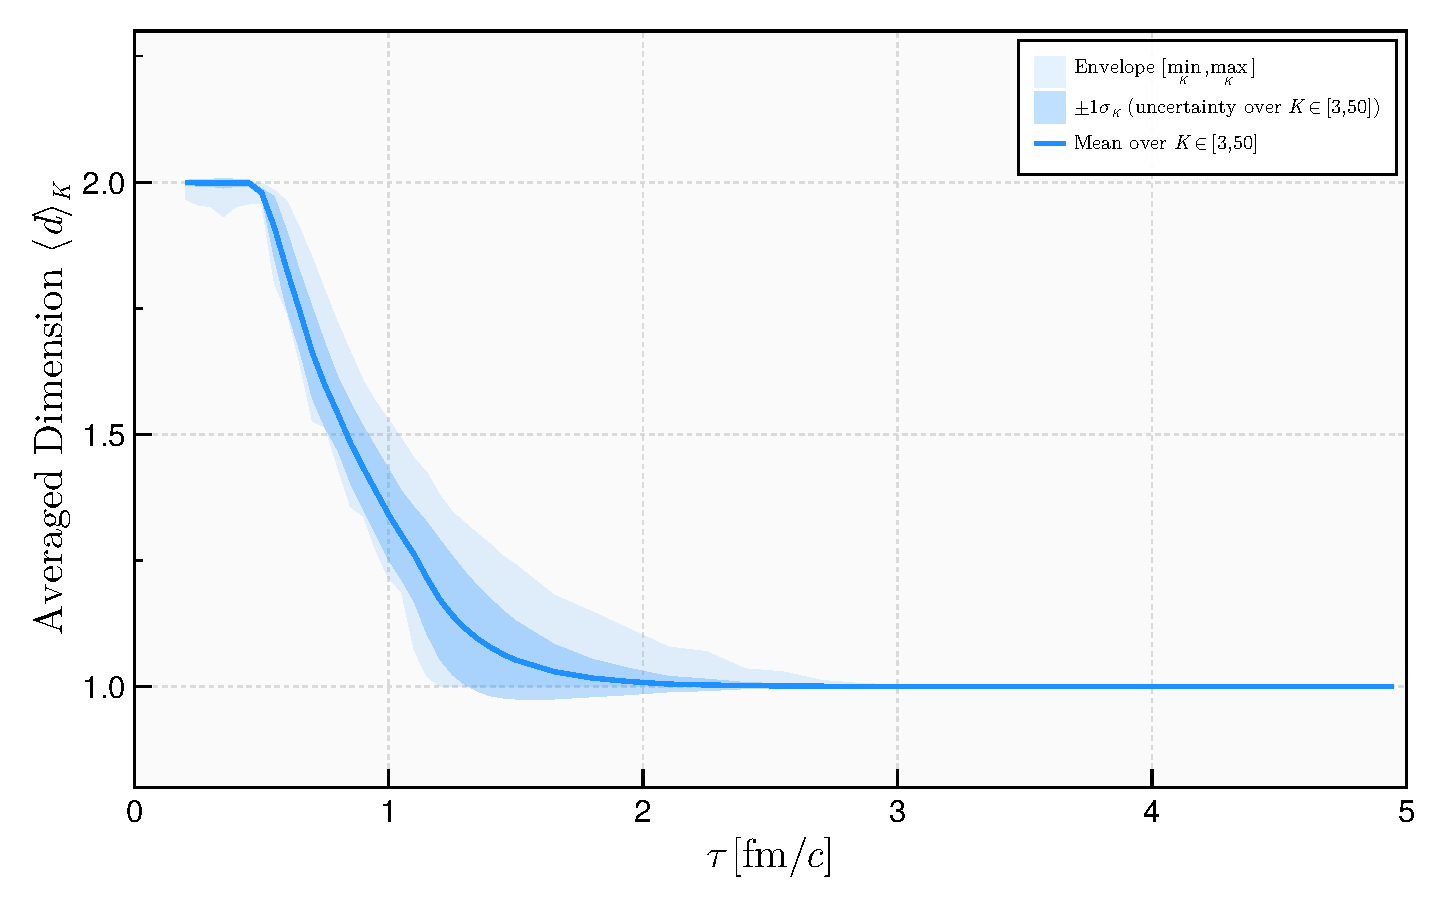
\includegraphics[width=\linewidth]{d_vs_tau_k_dependency/d_vs_tau_mis_minmax_k_averaged_dims.pdf}
        \caption{MIS: Min-Max}
    \end{subfigure}
    \hfill
    \begin{subfigure}[b]{0.32\textwidth}
        \centering
        \includegraphics[width=\linewidth]{d_vs_tau_k_dependency/d_vs_tau_mis_max_k_averaged_dims.pdf}
        \caption{MIS: Abs-Max}
    \end{subfigure}

    \vspace{0.8em}

    \begin{subfigure}[b]{0.32\textwidth}
        \centering
        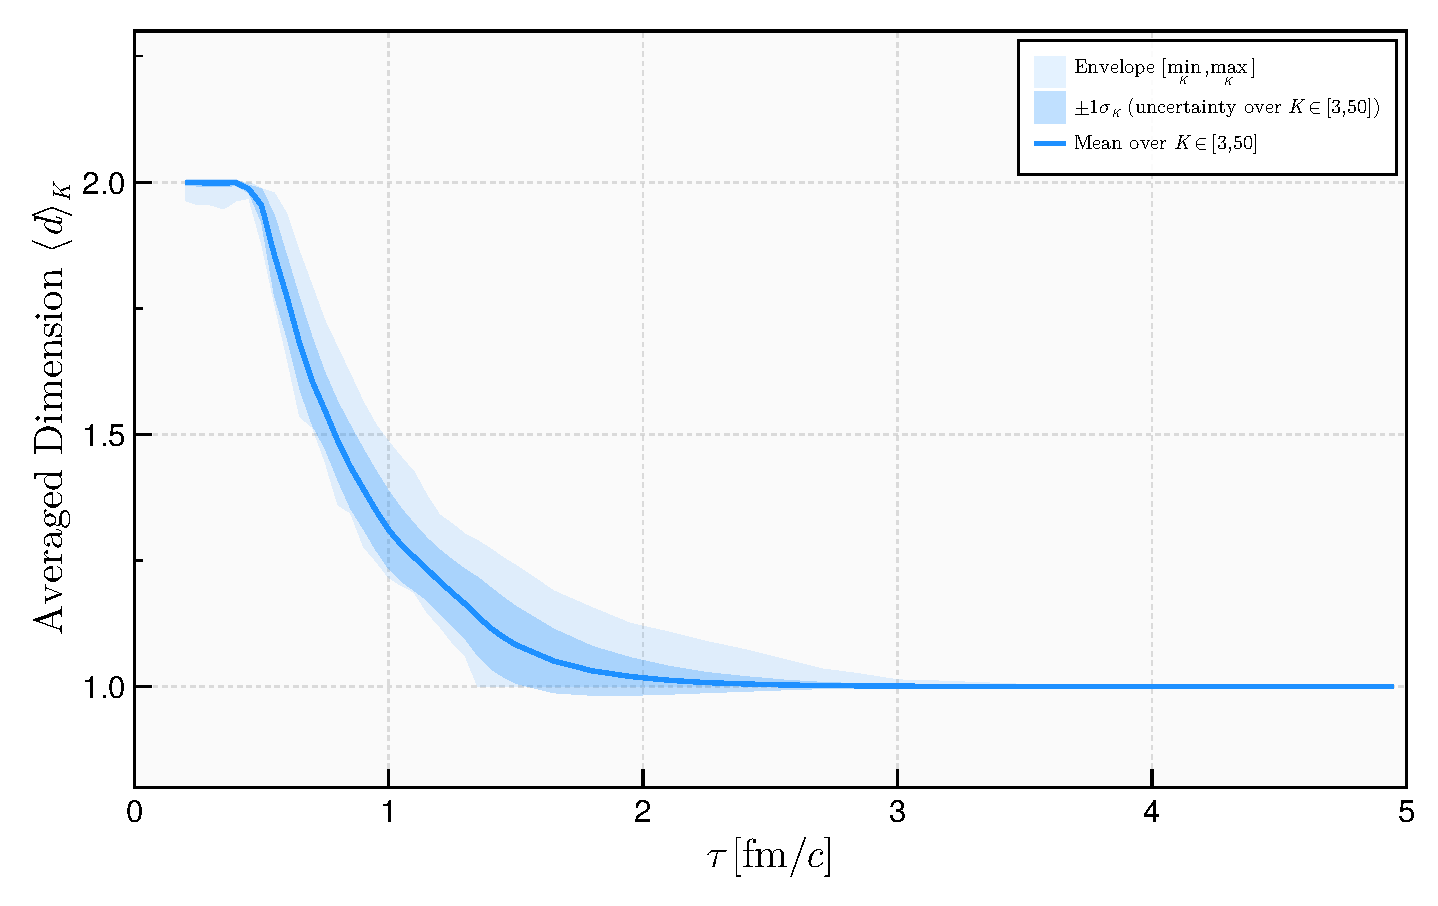
\includegraphics[width=\linewidth]{d_vs_tau_k_dependency/d_vs_tau_mis_physical_k_averaged_dims.pdf}
        \caption{MIS: Physical (brak stand.)}
    \end{subfigure}
    \hspace{0.05\textwidth}
    \begin{subfigure}[b]{0.32\textwidth}
        \centering
        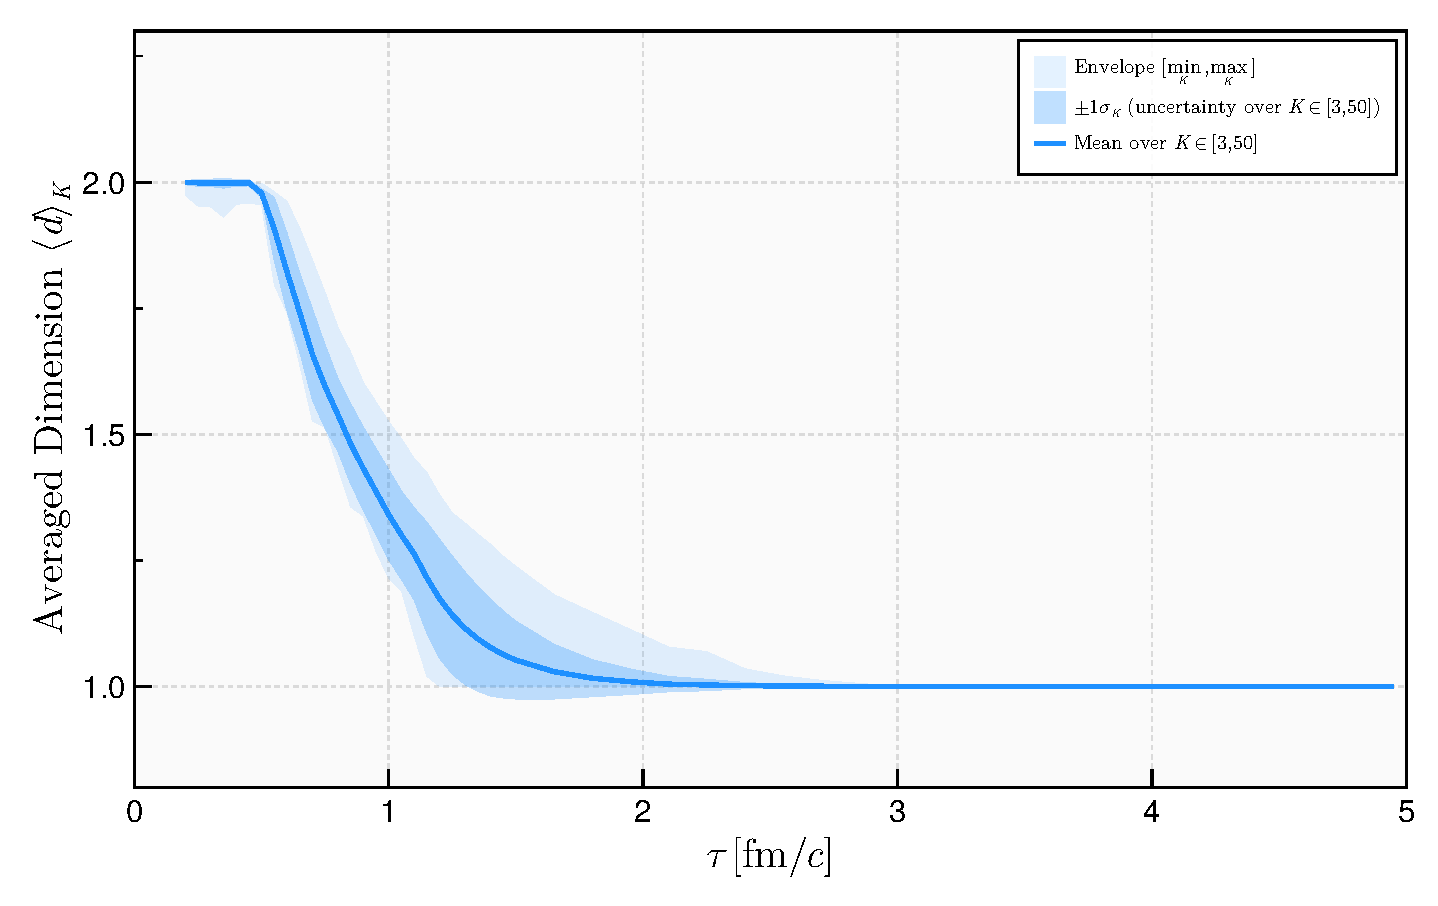
\includegraphics[width=\linewidth]{d_vs_tau_k_dependency/d_vs_tau_mis_dimensionless_k_averaged_dims.pdf}
        \caption{MIS: Dimensionless}
    \end{subfigure}

    \caption{Porównanie ewolucji uśrednionego wymiaru $\langle d \rangle_K(\tau)$ (\emph{dims}) w modelu Conformal MIS dla 5 metod standaryzacji przestrzeni fazowej. Wszystkie znormalizowane metody jednoznacznie identyfikują atraktor 1D, podczas gdy brak standaryzacji (Physical) prowadzi do artefaktów skali wymiarowej.}
    \label{fig:d_tau_mis_all_standardizations}
\end{figure}

\begin{figure}[htbp]
    \centering
    \begin{subfigure}[b]{0.32\textwidth}
        \centering
        \includegraphics[width=\linewidth]{d_vs_tau_k_dependency/d_vs_tau_hjsw_zscore_k_averaged_dims.pdf}
        \caption{HJSW: Z-Score}
    \end{subfigure}
    \hfill
    \begin{subfigure}[b]{0.32\textwidth}
        \centering
        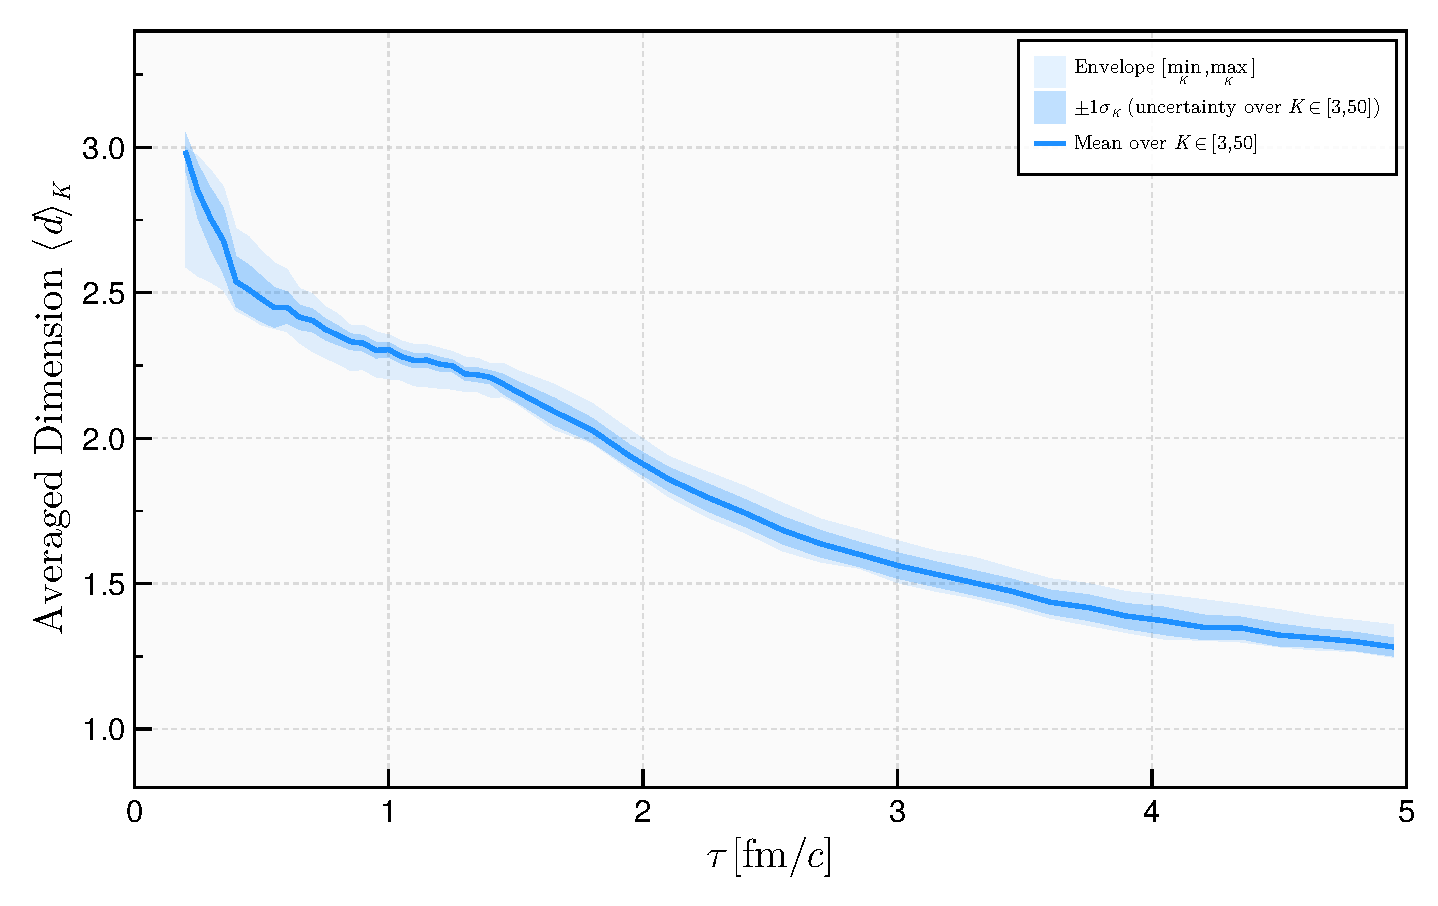
\includegraphics[width=\linewidth]{d_vs_tau_k_dependency/d_vs_tau_hjsw_minmax_k_averaged_dims.pdf}
        \caption{HJSW: Min-Max}
    \end{subfigure}
    \hfill
    \begin{subfigure}[b]{0.32\textwidth}
        \centering
        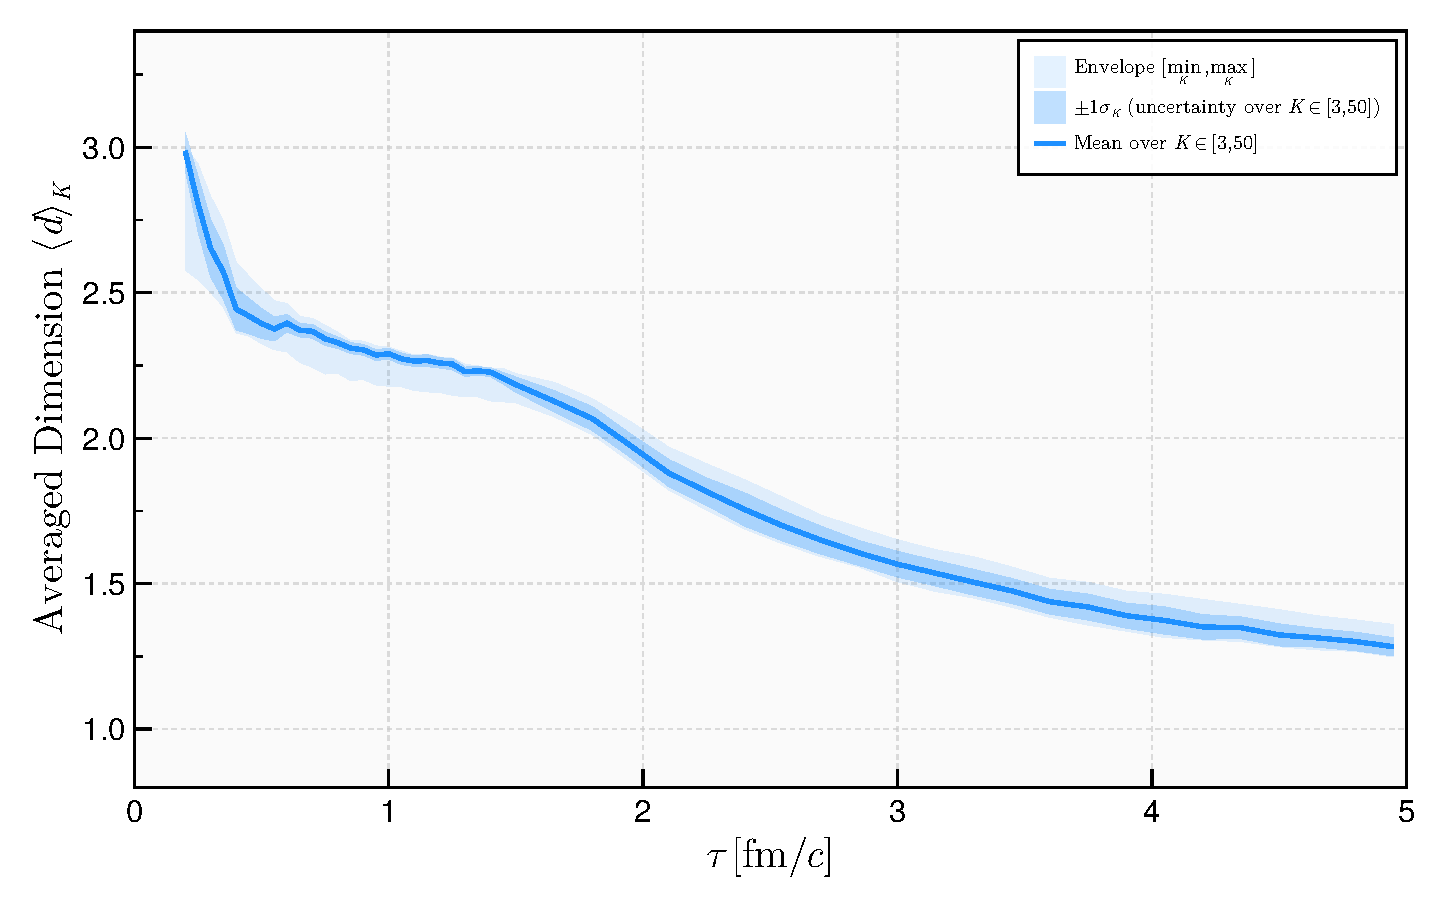
\includegraphics[width=\linewidth]{d_vs_tau_k_dependency/d_vs_tau_hjsw_max_k_averaged_dims.pdf}
        \caption{HJSW: Abs-Max}
    \end{subfigure}

    \vspace{0.8em}

    \begin{subfigure}[b]{0.32\textwidth}
        \centering
        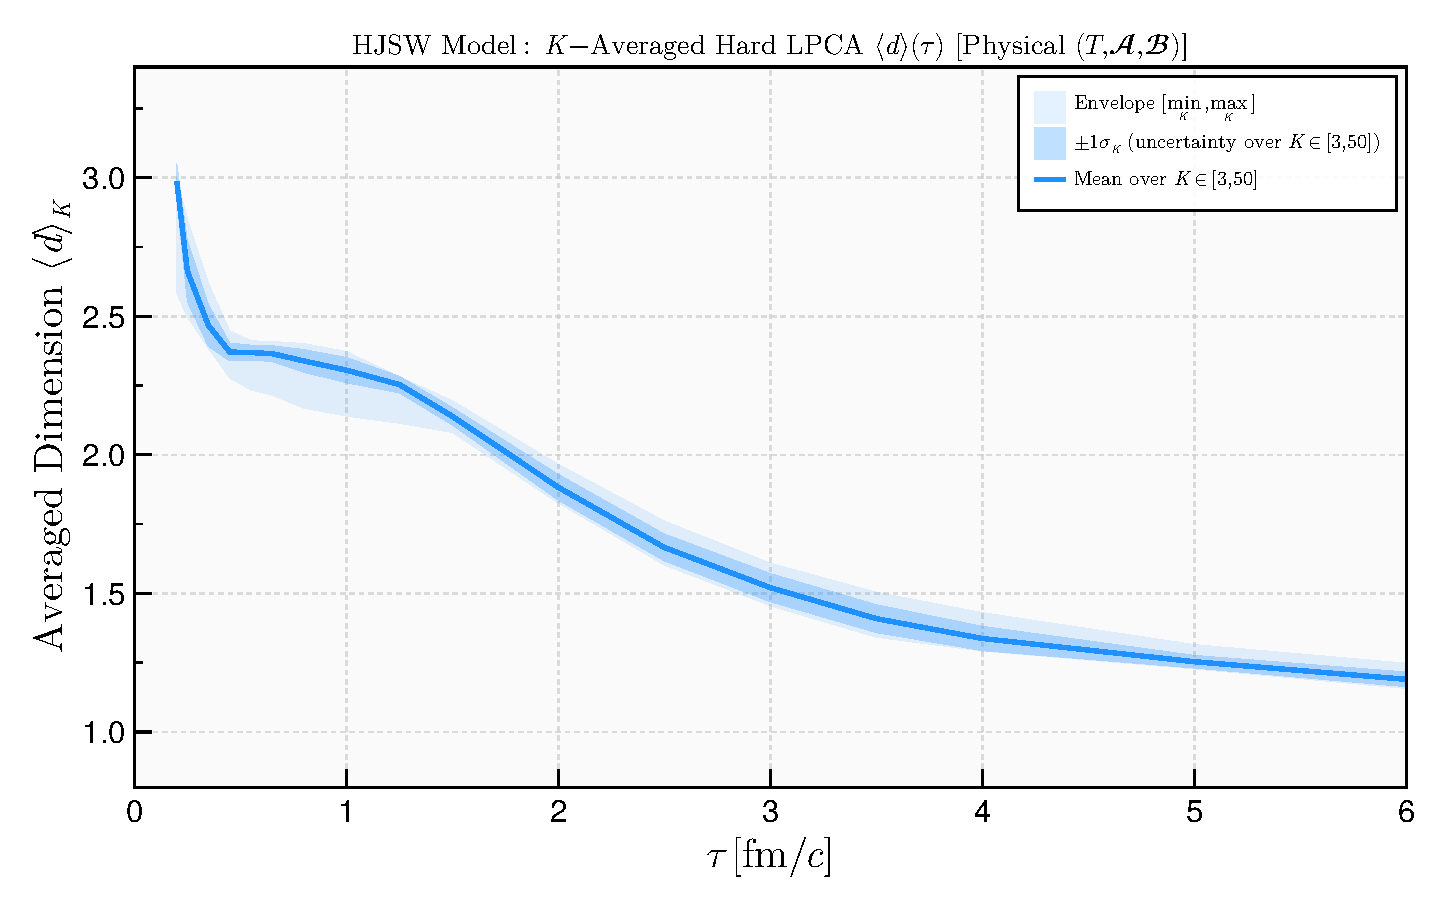
\includegraphics[width=\linewidth]{d_vs_tau_k_dependency/d_vs_tau_hjsw_physical_k_averaged_dims.pdf}
        \caption{HJSW: Physical (brak stand.)}
    \end{subfigure}
    \hspace{0.05\textwidth}
    \begin{subfigure}[b]{0.32\textwidth}
        \centering
        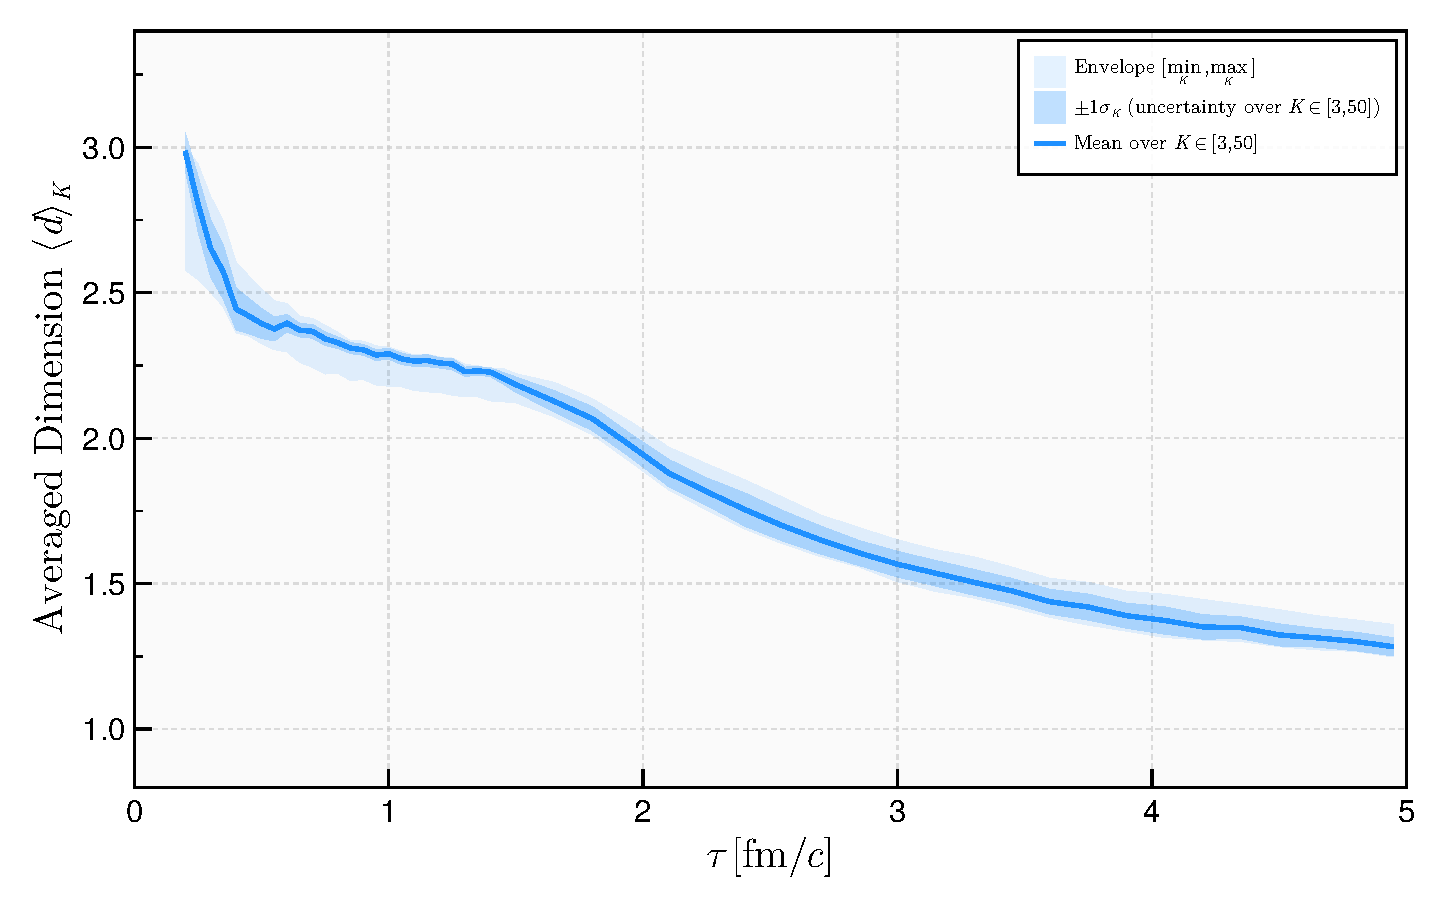
\includegraphics[width=\linewidth]{d_vs_tau_k_dependency/d_vs_tau_hjsw_dimensionless_k_averaged_dims.pdf}
        \caption{HJSW: Dimensionless}
    \end{subfigure}

    \caption{Porównanie ewolucji uśrednionego wymiaru $\langle d \rangle_K(\tau)$ (\emph{dims}) w modelu HJSW dla 5 metod standaryzacji przestrzeni fazowej. Metody Z-Score, Min-Max, Abs-Max oraz Dimensionless poprawnie rejestrują hierarchiczny kolaps $3 \to 2 \to 1$, natomiast współrzędne fizyczne bez normalizacji tłumią widoczność rozmaitości pośredniej 2D.}
    \label{fig:d_tau_hjsw_all_standardizations}
\end{figure}

\clearpage
\section{Kategoria III: Zależność wymiaru od wielkości otoczenia $d(K)$}

\begin{figure}[htbp]
    \centering
    \begin{subfigure}[b]{0.48\textwidth}
        \centering
        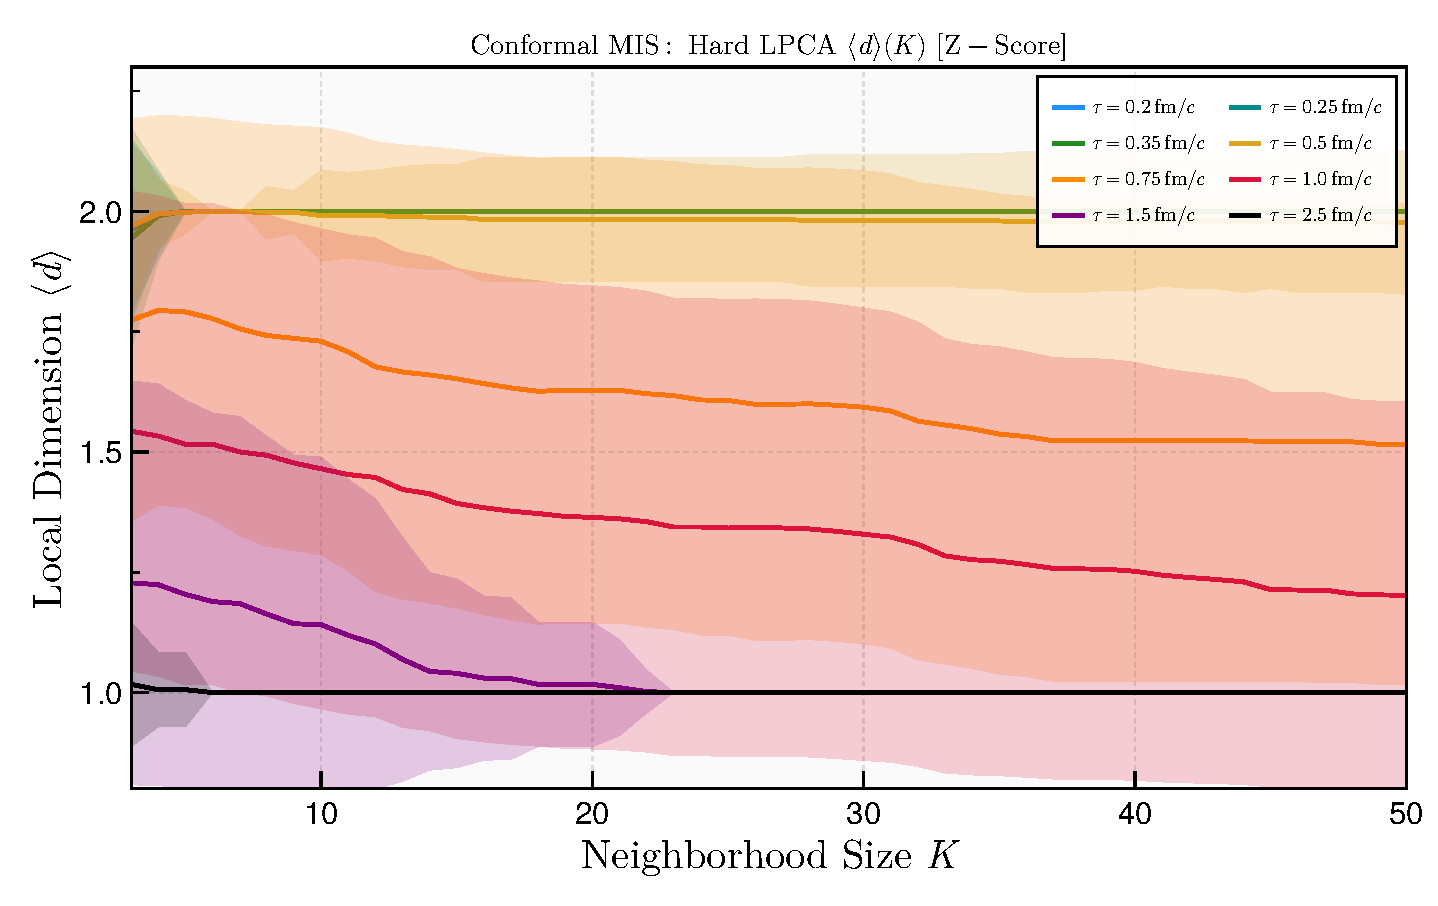
\includegraphics[width=\linewidth]{k_sweep_curves/k_sweep_mis_zscore_dims.pdf}
        \caption{MIS: \emph{dims} w funkcji $K$}
        \label{fig:k_sweep_mis_dims}
    \end{subfigure}
    \hfill
    \begin{subfigure}[b]{0.48\textwidth}
        \centering
        \includegraphics[width=\linewidth]{k_sweep_curves/k_sweep_mis_zscore_pr.pdf}
        \caption{MIS: \emph{pr} w funkcji $K$}
        \label{fig:k_sweep_mis_pr}
    \end{subfigure}

    \vspace{0.8em}

    \begin{subfigure}[b]{0.48\textwidth}
        \centering
        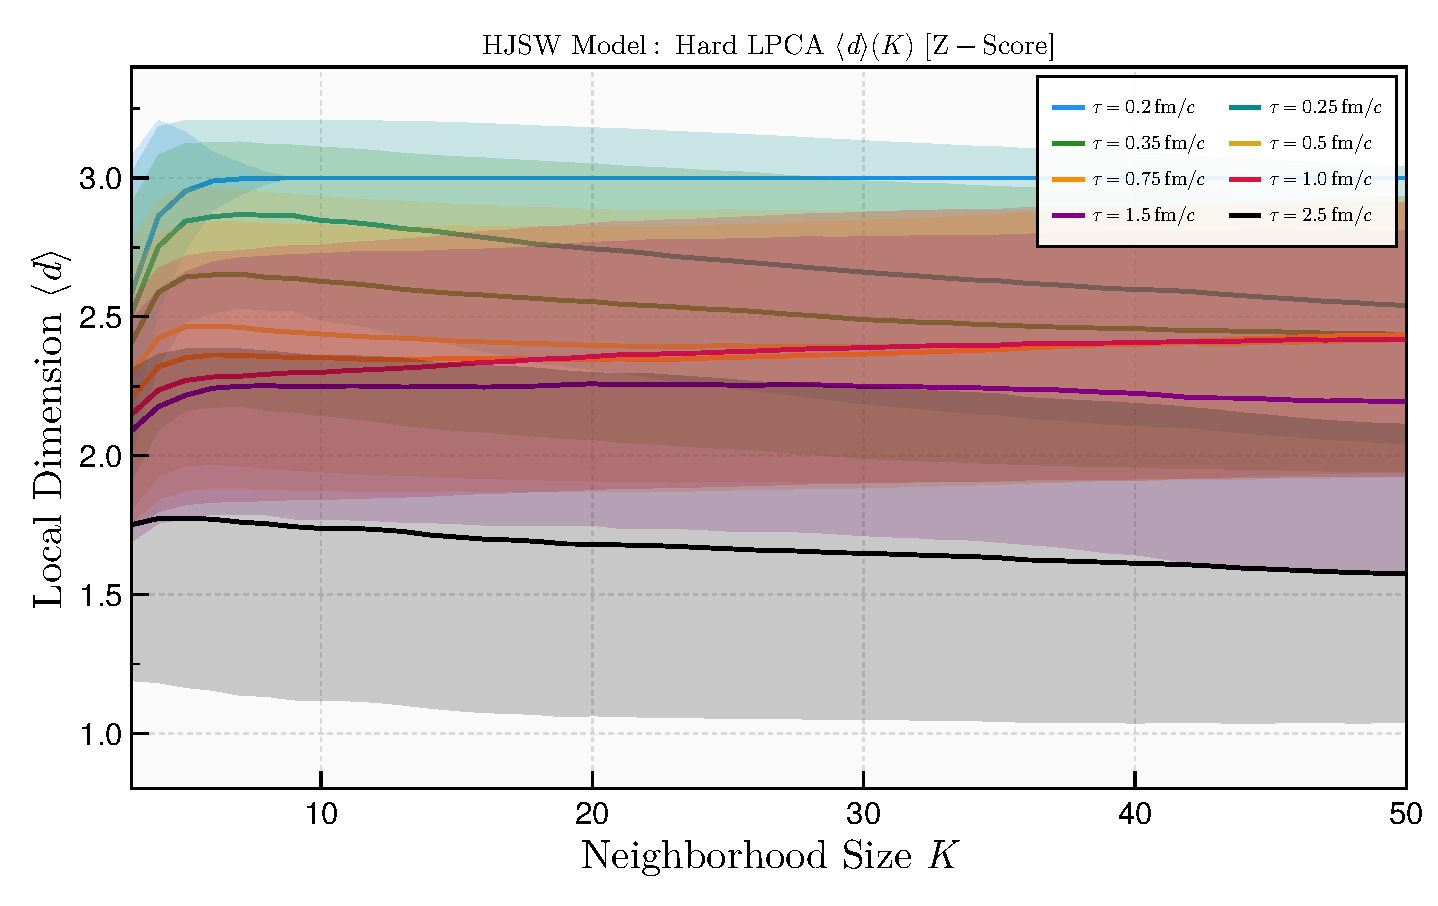
\includegraphics[width=\linewidth]{k_sweep_curves/k_sweep_hjsw_zscore_dims.pdf}
        \caption{HJSW: \emph{dims} w funkcji $K$}
        \label{fig:k_sweep_hjsw_dims}
    \end{subfigure}
    \hfill
    \begin{subfigure}[b]{0.48\textwidth}
        \centering
        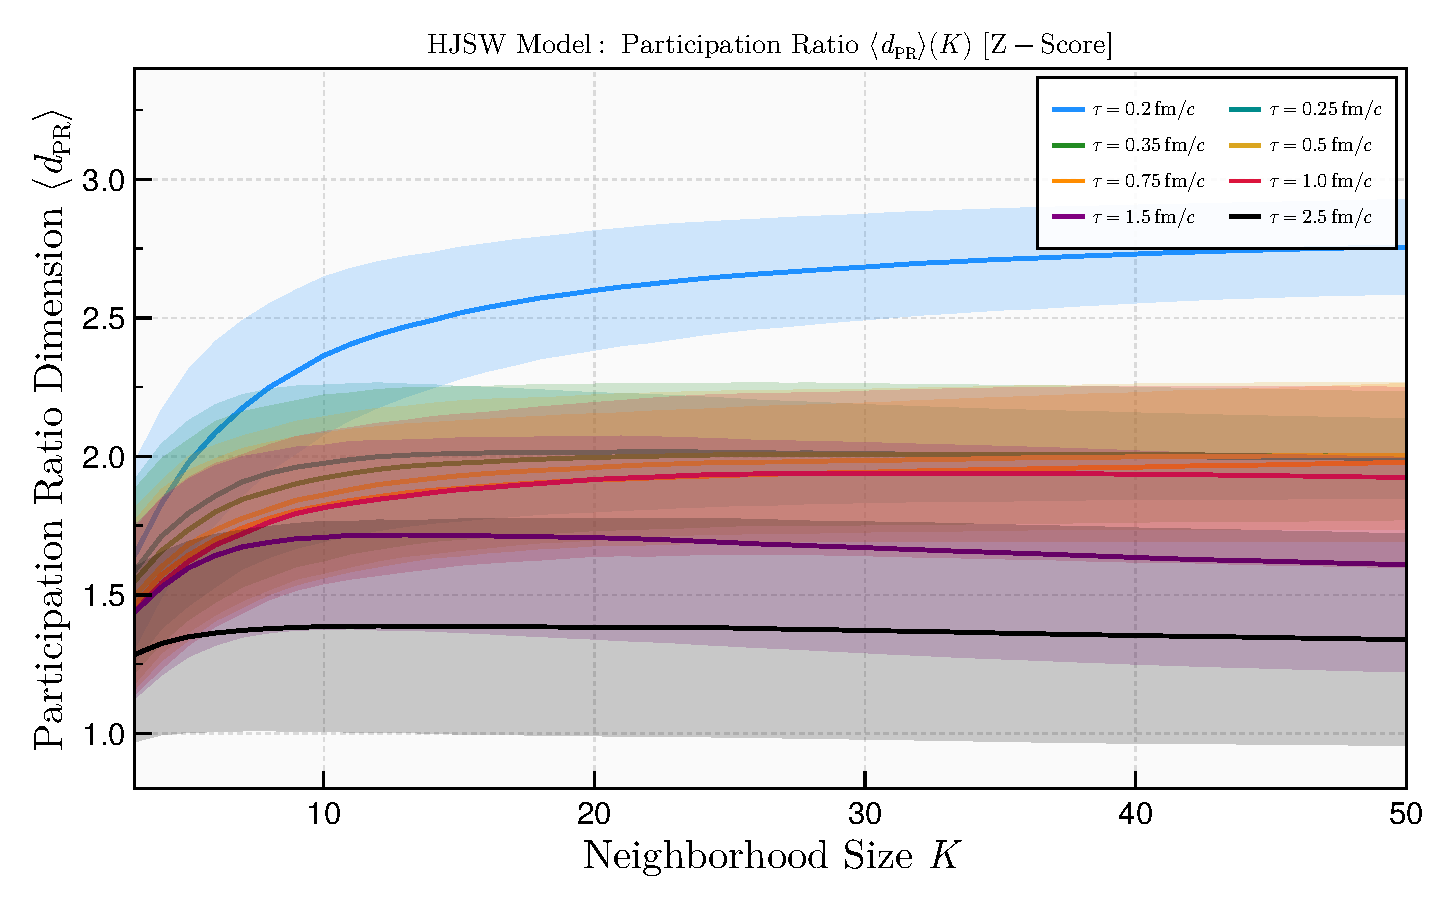
\includegraphics[width=\linewidth]{k_sweep_curves/k_sweep_hjsw_zscore_pr.pdf}
        \caption{HJSW: \emph{pr} w funkcji $K$}
        \label{fig:k_sweep_hjsw_pr}
    \end{subfigure}

    \caption{Zależność wymiaru lokalnego od wielkości otoczenia $K \in [3, 50]$ w standaryzacji Z-Score dla 8 wybranych przekrojów $\tau \in [0.20, 2.50]\,\mathrm{fm}/c$. Płaskowyż stabilności w szerokim przedziale $K \in [10, 40]$ potwierdza odporność procedury LPCA na wybór parametru skali sąsiedztwa.}
    \label{fig:k_sweep_curves_main}
\end{figure}

\end{document}

